% !TeX root = ../../Skript.tex
\cohead{\Large\textbf{Schaubilder der Ableitungsfunktion}}
\fakesubsection{Schaubilder der Ableitungsfunktion}
\begin{minipage}{\textwidth}
	\adjustbox{valign=t, padding = 0ex 0ex 2ex 0ex}{\begin{minipage}{0.5\textwidth-2ex}
		\centering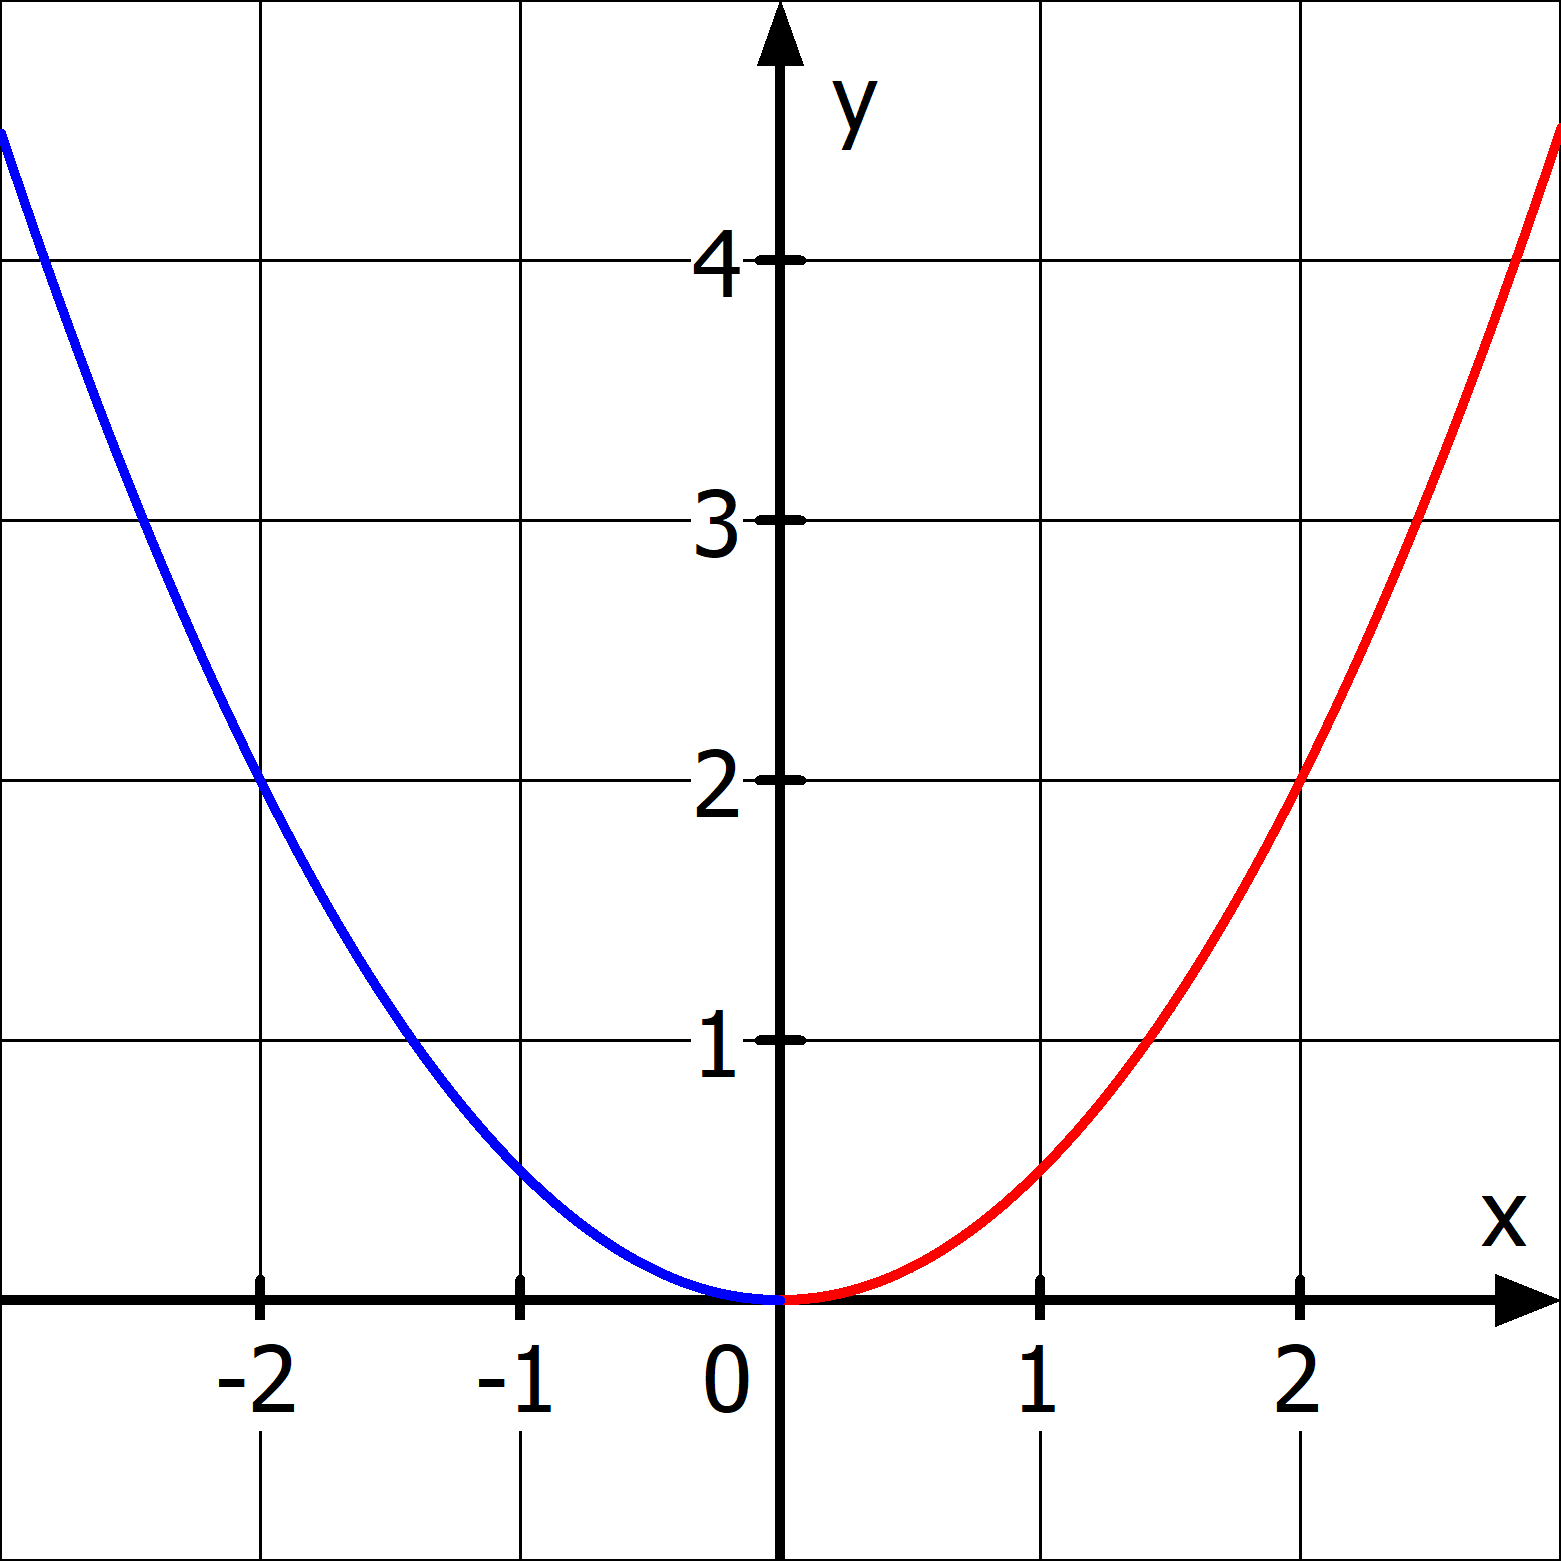
\includegraphics[width=\textwidth]{\ableitung/pics/ablSchaubild1.png}

		\(f(x)=0,5x^2\)
	\end{minipage}}%
	\adjustbox{valign=t, padding = 2ex 0ex 0ex 0ex}{\begin{minipage}{0.5\textwidth-2ex}
		\centering\includegraphics[width=\textwidth]{\ableitung/pics/x\iftoggle{ausfuellen}{}{_empty}.png}\\
		\(f'(x)=\textcolor{loes}{x}\)
	\end{minipage}}%
\end{minipage}

Das Schaubild von \(f(x)=x^2\) fällt für \(x<0\), d.h. alle Tangenten in diesem Bereich haben eine negative Steigung und damit ist die Ableitung negativ. Analog gilt für \(x>0\), dass das Schaubild steigt und damit die Ableitung positiv ist.

\begin{Exercise}[title={\raggedright Markiere jeweils in welchen Bereichen das Schaubild der Funktionen steigt bzw. fällt, die Ableitungen negativ bzw. positiv sind und ordne dann die Schaubilder der Funktioinen den passenden Schaubildern der Ableitungen zu.}, label=schaubildZuordnenA1]

\begin{minipage}{\textwidth}
	\begin{minipage}{0.5\textwidth}
		\centering Funktionen
	\end{minipage}%
	\begin{minipage}{0.5\textwidth}
		\centering Ableitungen
	\end{minipage}%
\end{minipage}

\begin{adjustbox}{max width=\textwidth}
    \adjustbox{valign=t, padding = 0ex 0ex 0ex 0ex }{%
        \begin{minipage}{0.25\textwidth}
            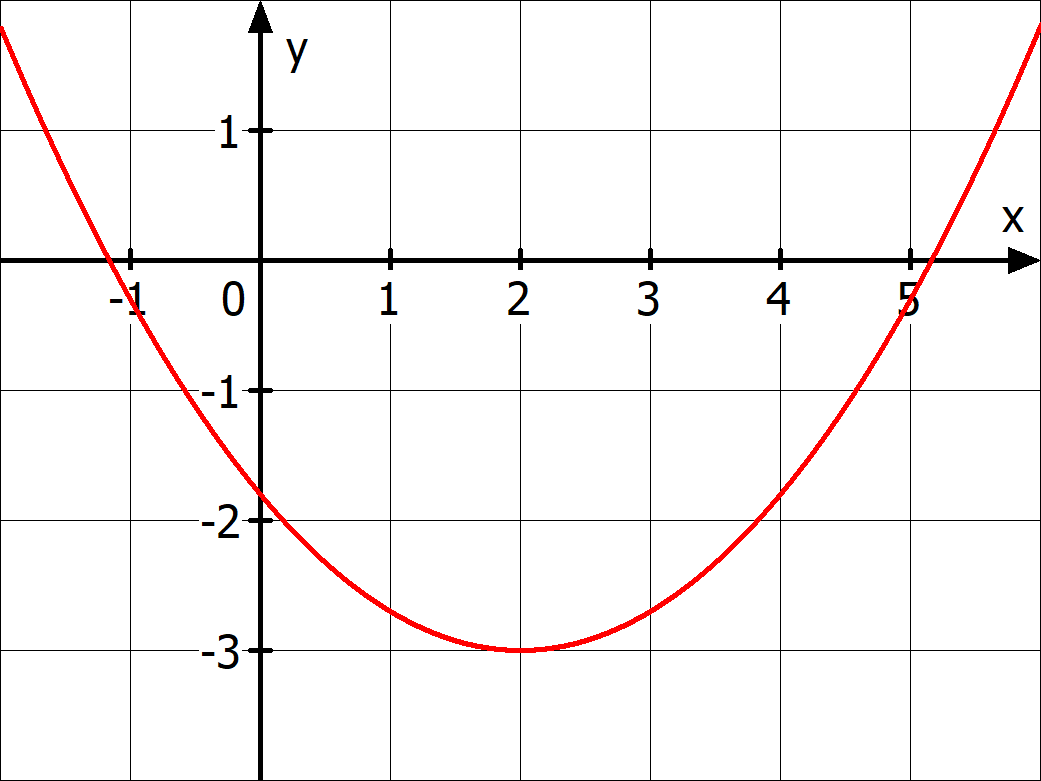
\includegraphics[width=\textwidth]{\ableitung/pics/zuordnenF1.png}%
        \end{minipage}}%
    \adjustbox{valign=t, padding = 2ex 0ex 0ex 0ex }{%
        \begin{minipage}{0.25\textwidth}
            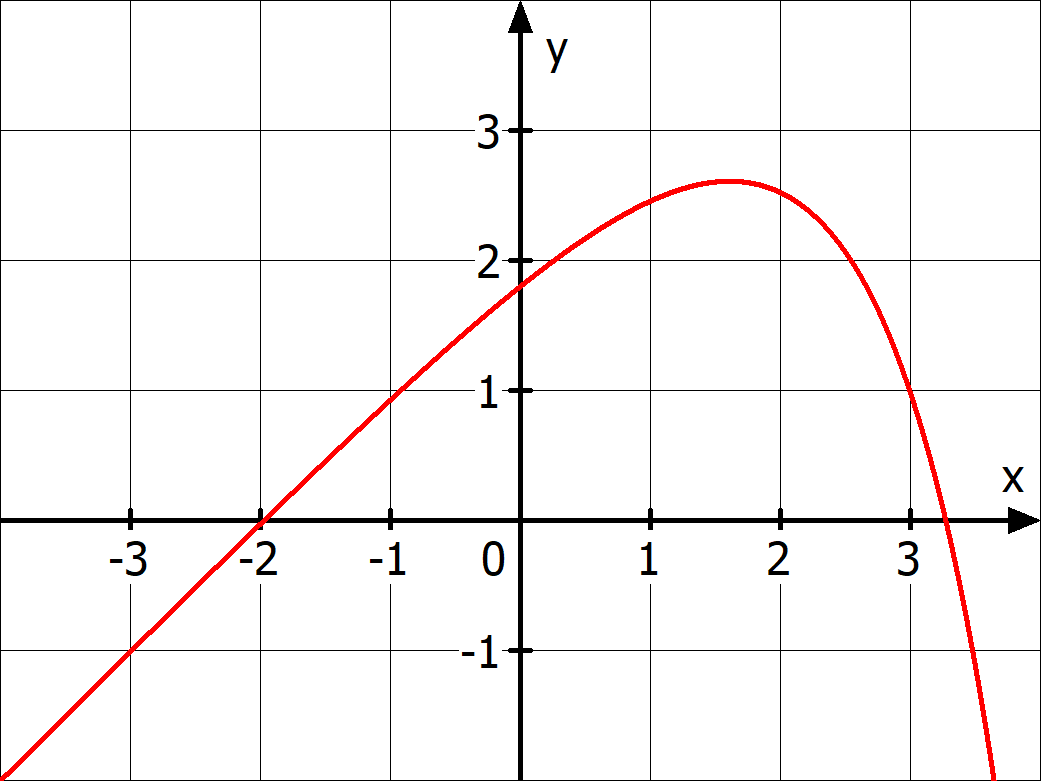
\includegraphics[width=\textwidth]{\ableitung/pics/zuordnenF6.png}%
        \end{minipage}}%
    \adjustbox{valign=t, padding = 4ex 0ex 0ex 0ex }{%
        \begin{minipage}{0.25\textwidth}
            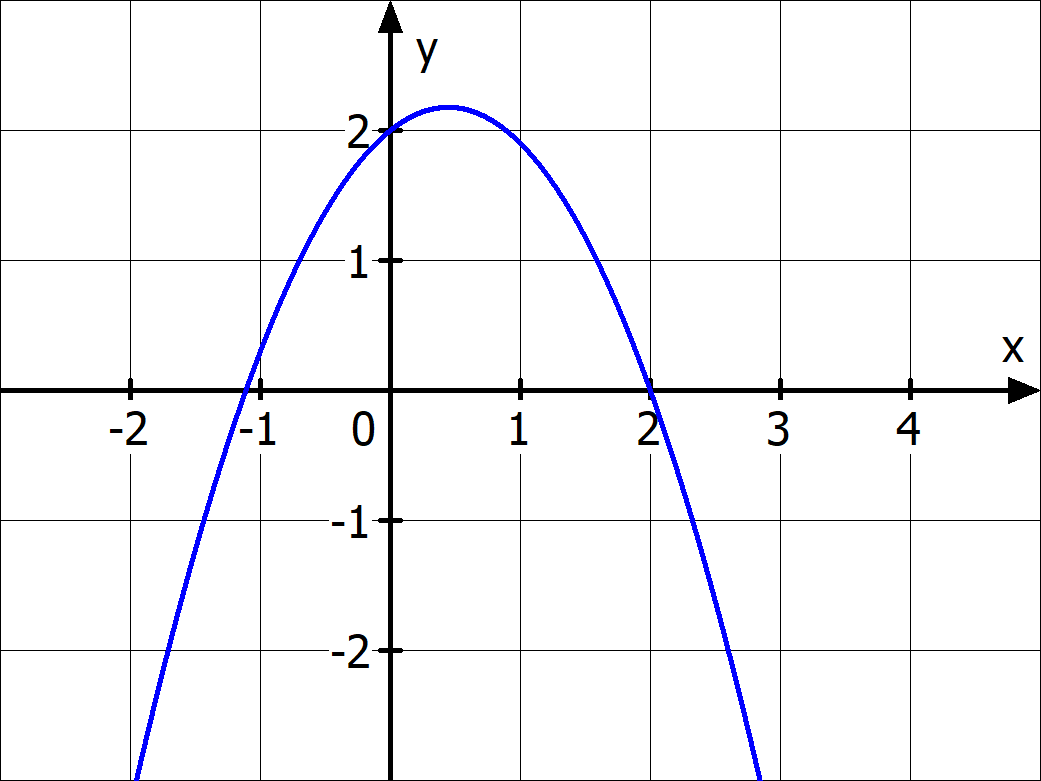
\includegraphics[width=\textwidth]{\ableitung/pics/zuordnenA4.png}%
           \end{minipage}}%
    \adjustbox{valign=t, padding = 2ex 0ex 0ex 0ex }{%
        \begin{minipage}{0.25\textwidth}
            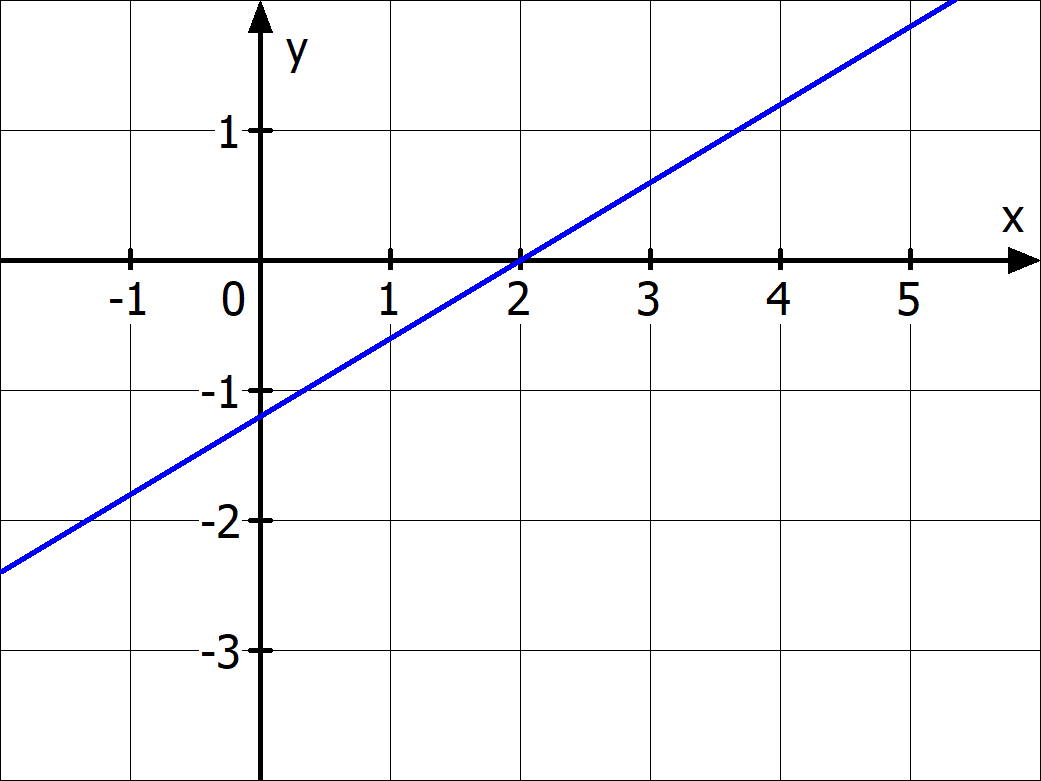
\includegraphics[width=\textwidth]{\ableitung/pics/zuordnenA1.png}%
        \end{minipage}}%
\end{adjustbox}%

\vspace{2ex}

\begin{adjustbox}{max width=\textwidth}
    \adjustbox{valign=t, padding = 0ex 0ex 0ex 0ex }{%
        \begin{minipage}{0.25\textwidth}
            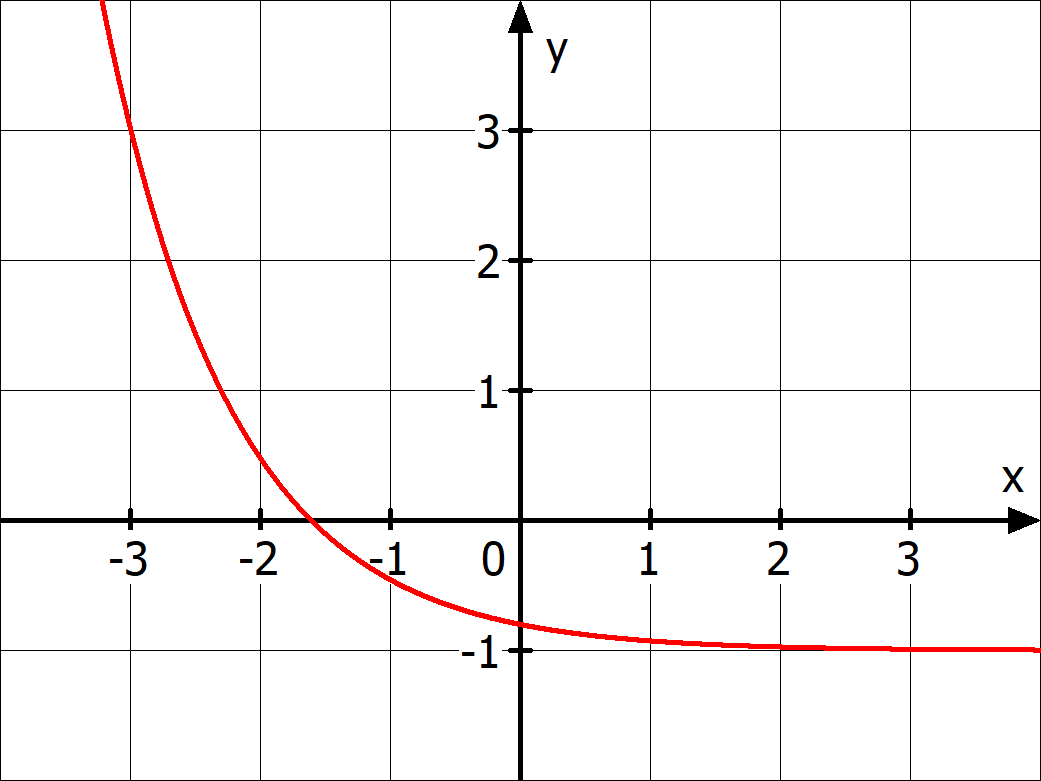
\includegraphics[width=\textwidth]{\ableitung/pics/zuordnenF3.png}%
    \end{minipage}}%
    \adjustbox{valign=t, padding = 2ex 0ex 0ex 0ex }{%
        \begin{minipage}{0.25\textwidth}
            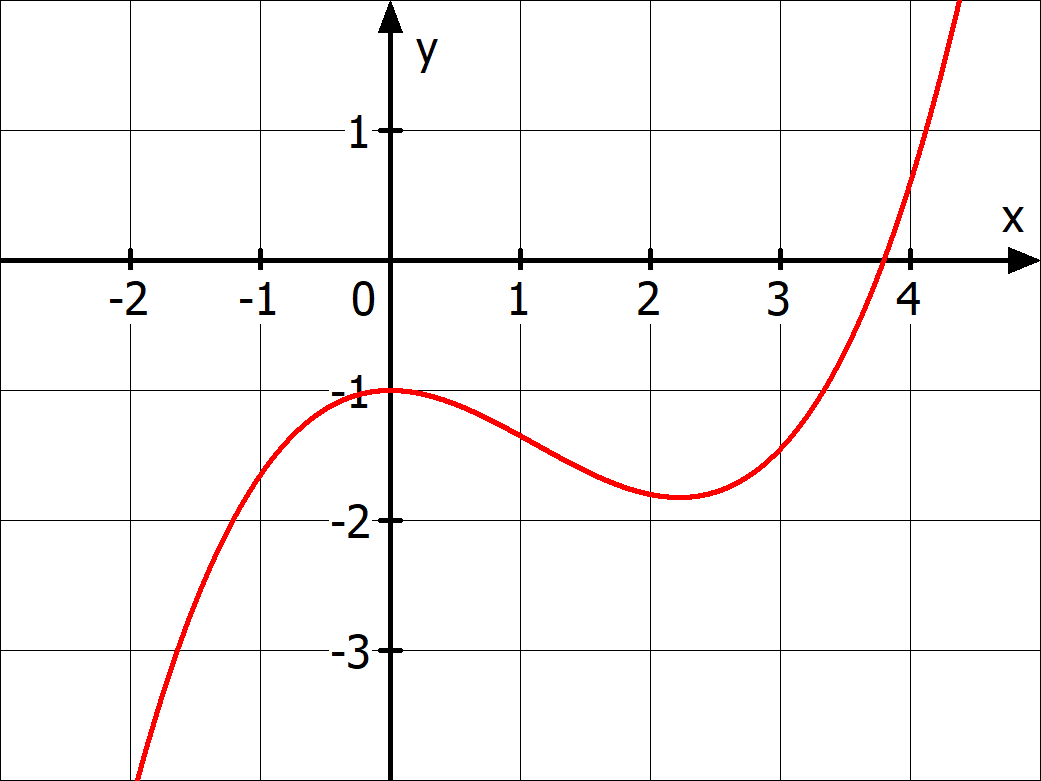
\includegraphics[width=\textwidth]{\ableitung/pics/zuordnenF2.png}%
    \end{minipage}}%
    \adjustbox{valign=t, padding = 4ex 0ex 0ex 0ex }{%
        \begin{minipage}{0.25\textwidth}
            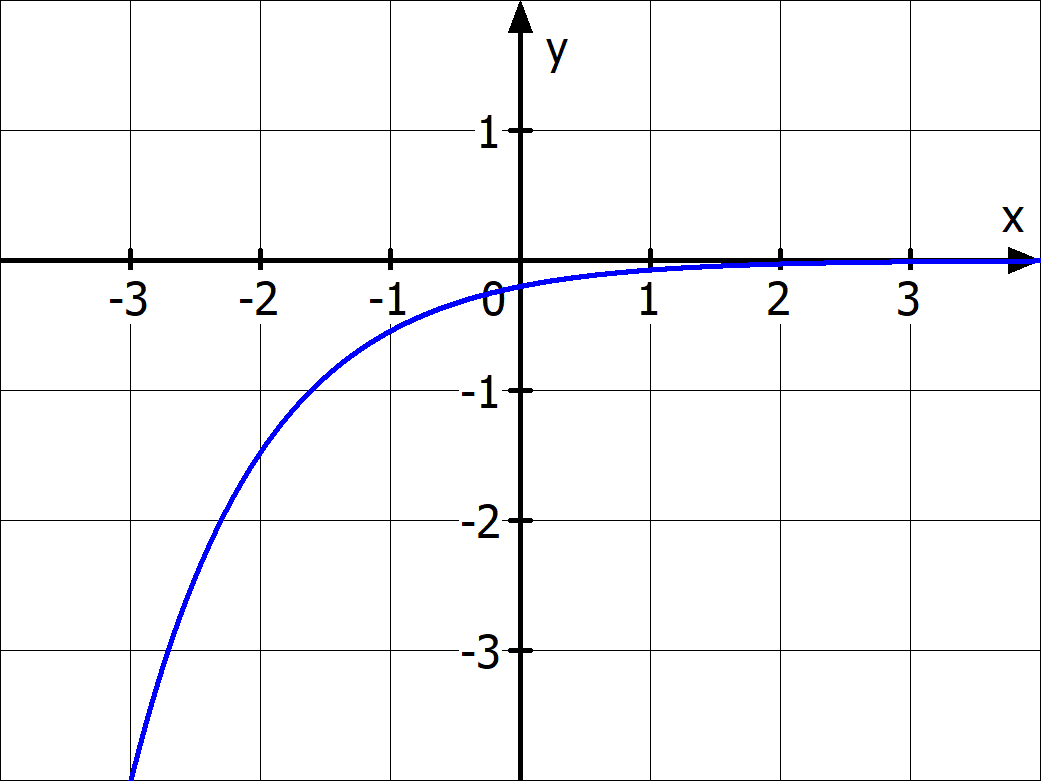
\includegraphics[width=\textwidth]{\ableitung/pics/zuordnenA3.png}%
    \end{minipage}}%
    \adjustbox{valign=t, padding = 2ex 0ex 0ex 0ex }{%
        \begin{minipage}{0.25\textwidth}
            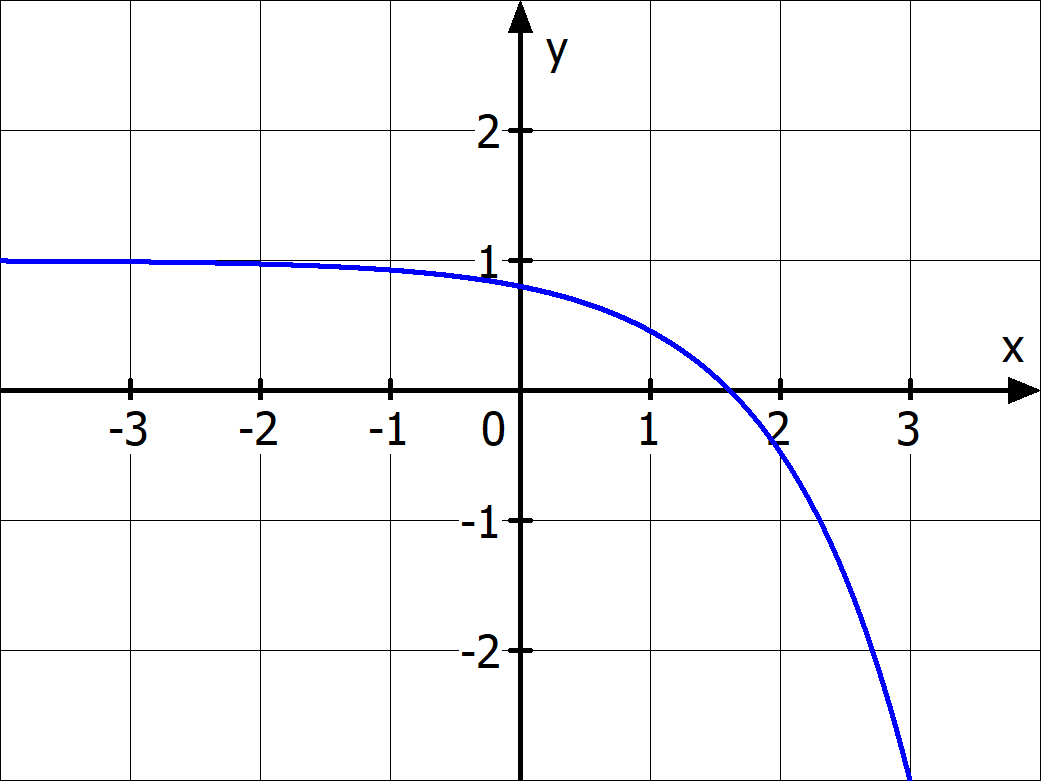
\includegraphics[width=\textwidth]{\ableitung/pics/zuordnenA6.png}%
    \end{minipage}}%
\end{adjustbox}%

\vspace{2ex}

\begin{adjustbox}{max width=\textwidth}%
    \adjustbox{valign=t, padding = 0ex 0ex 0ex 0ex }{%
        \begin{minipage}{0.25\textwidth}
            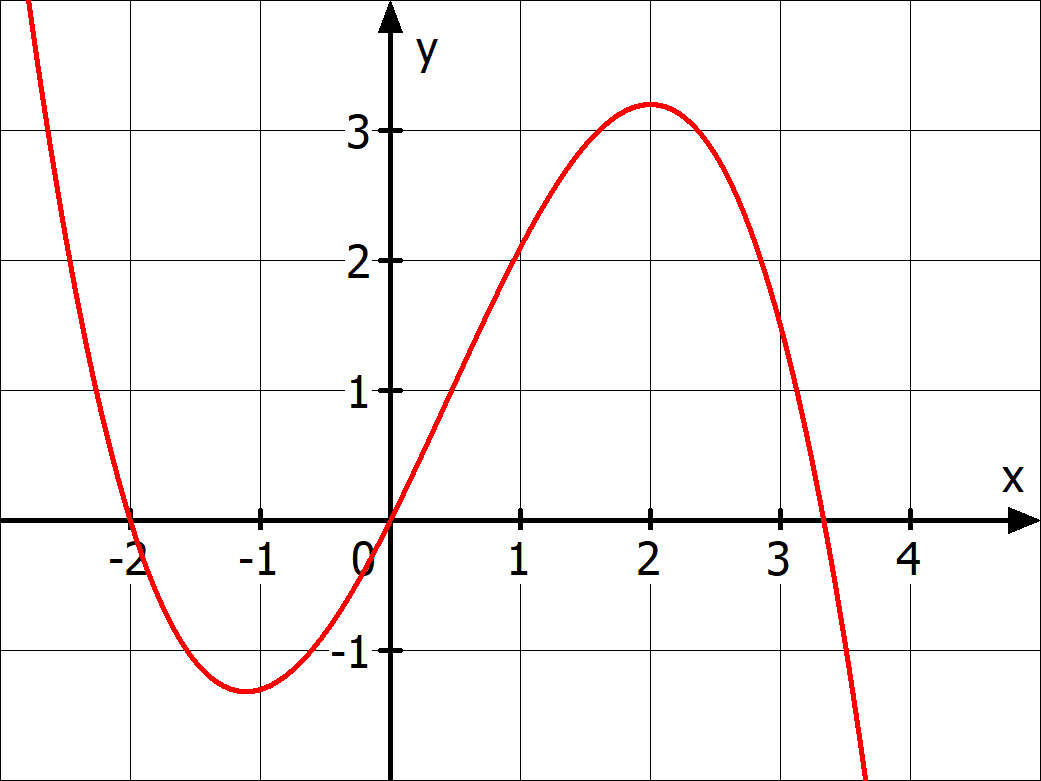
\includegraphics[width=\textwidth]{\ableitung/pics/zuordnenF4.png}%
    \end{minipage}}%
    \adjustbox{valign=t, padding = 2ex 0ex 0ex 0ex }{%
        \begin{minipage}{0.25\textwidth}
            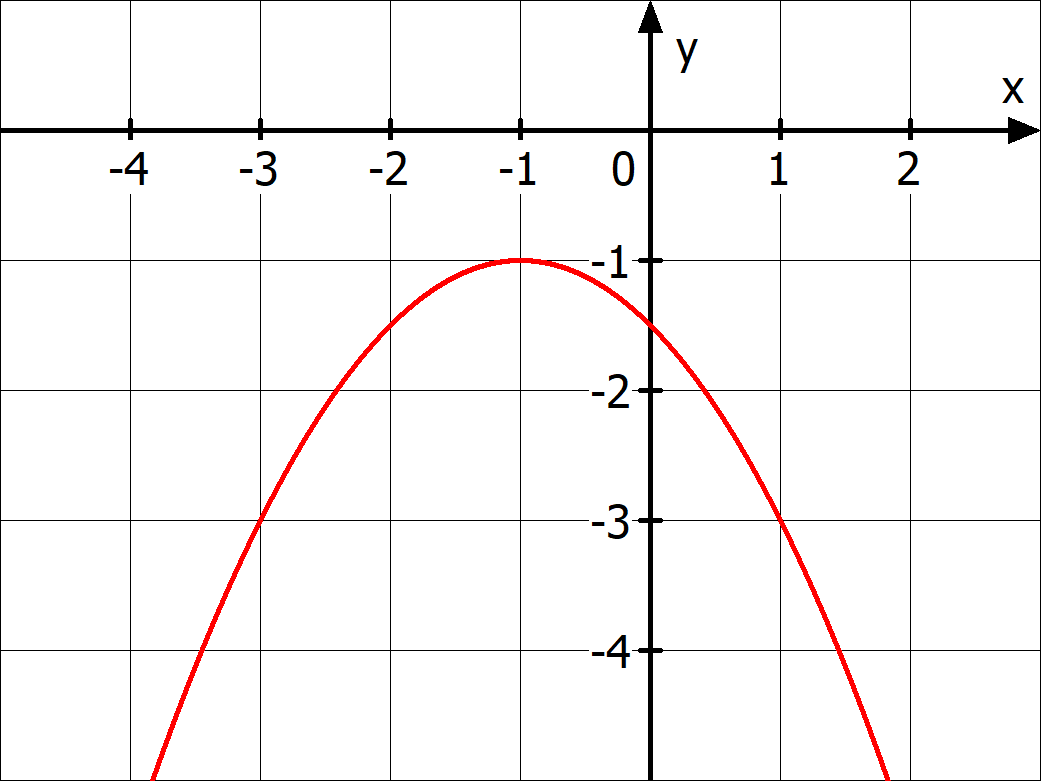
\includegraphics[width=\textwidth]{\ableitung/pics/zuordnenF5.png}%
    \end{minipage}}%
    \adjustbox{valign=t, padding = 4ex 0ex 0ex 0ex }{%
        \begin{minipage}{0.25\textwidth}
            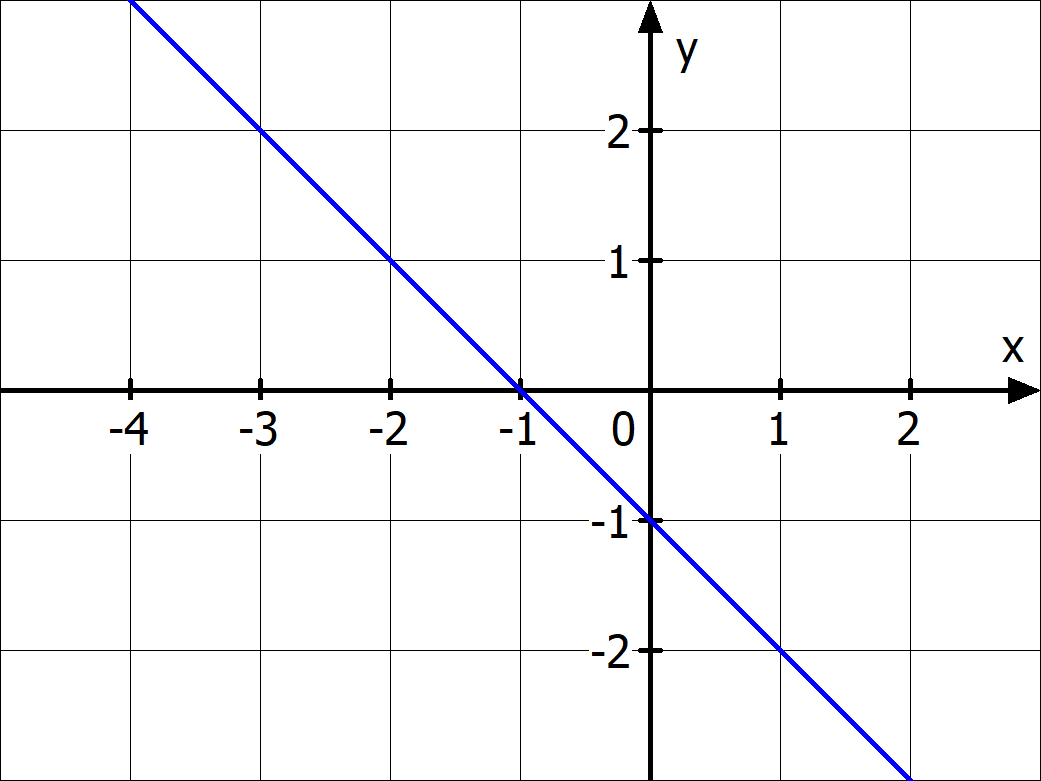
\includegraphics[width=\textwidth]{\ableitung/pics/zuordnenA5.png}%
    \end{minipage}}%
    \adjustbox{valign=t, padding = 2ex 0ex 0ex 0ex }{%
        \begin{minipage}{0.25\textwidth}
            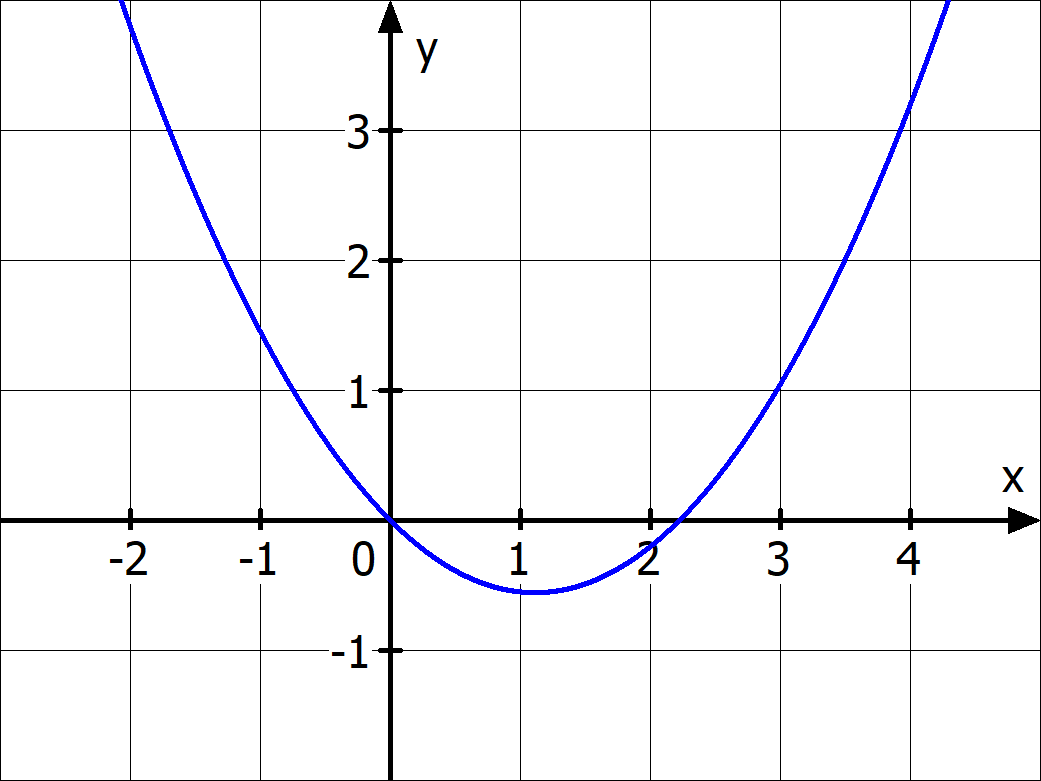
\includegraphics[width=\textwidth]{\ableitung/pics/zuordnenA2.png}%
    \end{minipage}}%
\end{adjustbox}%
\end{Exercise}%
\newpage
\begin{Exercise}[title={\raggedright Skizziere jeweils die Ableitungsfunktion.}, label=ableitungSkizzierenA1]

	\begin{minipage}{\textwidth}
		\begin{minipage}{0.5\textwidth}
			\centering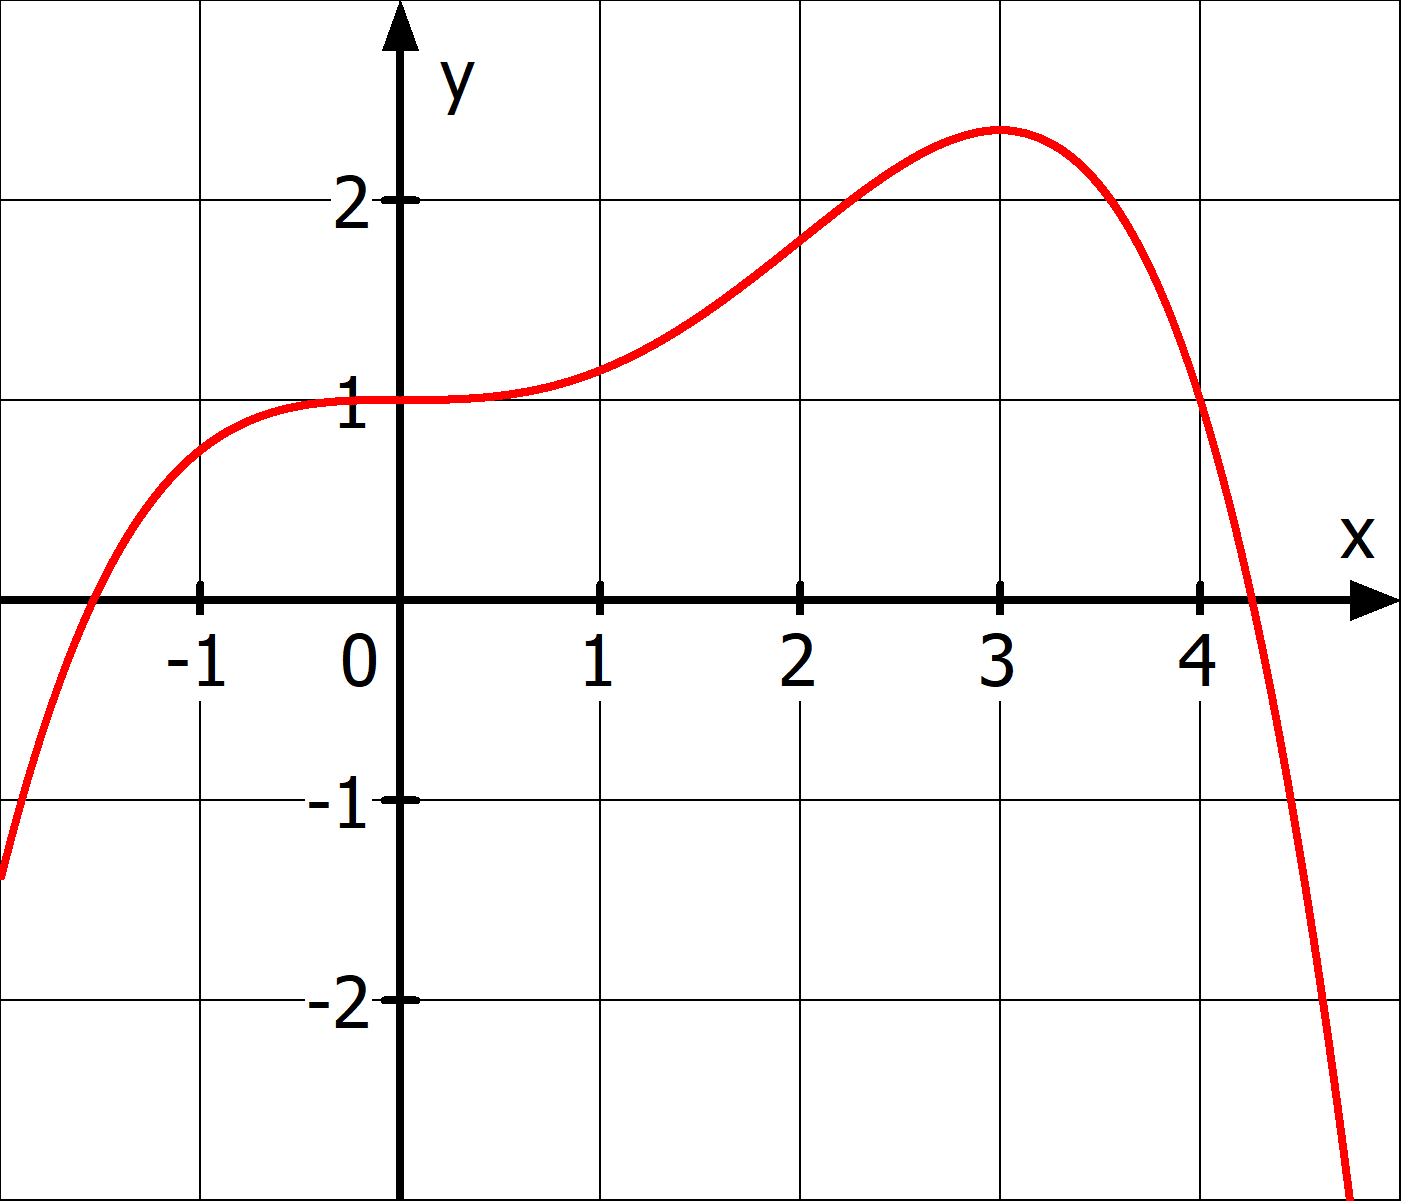
\includegraphics[width=.8\textwidth]{\ableitung/pics/ablSkizzierenF1.png}

            \vspace{0.1cm}

			\centering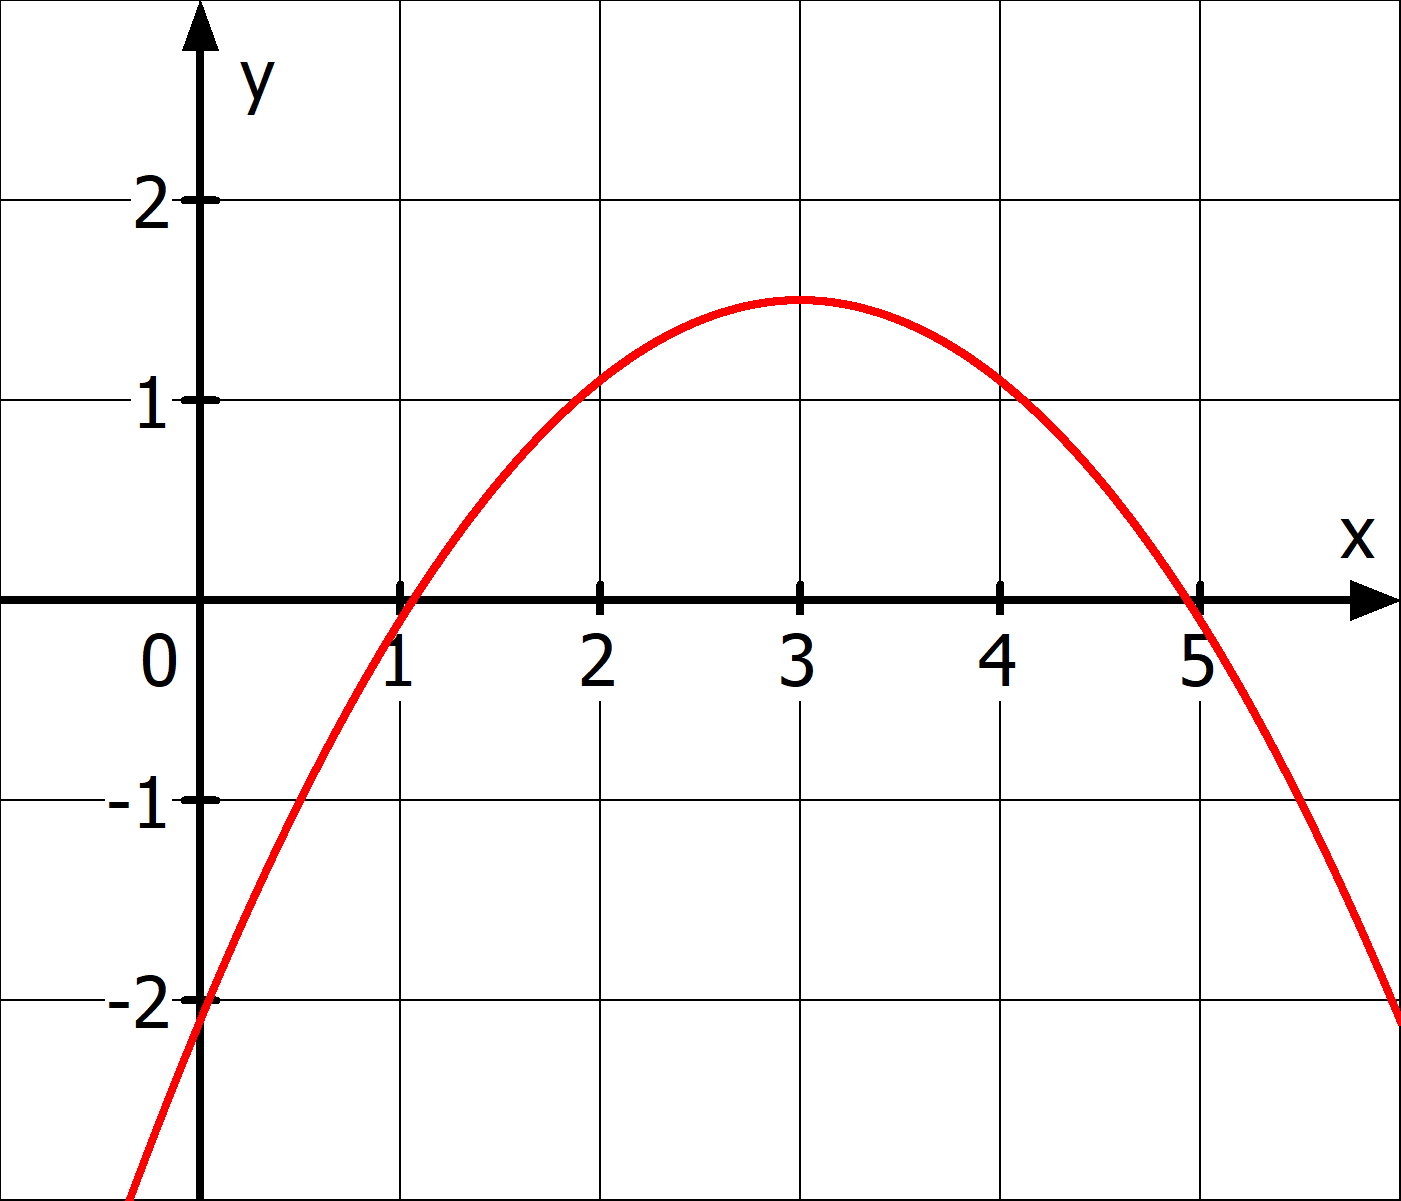
\includegraphics[width=.8\textwidth]{\ableitung/pics/ablSkizzierenF2.png}

            \vspace{0.1cm}

			\centering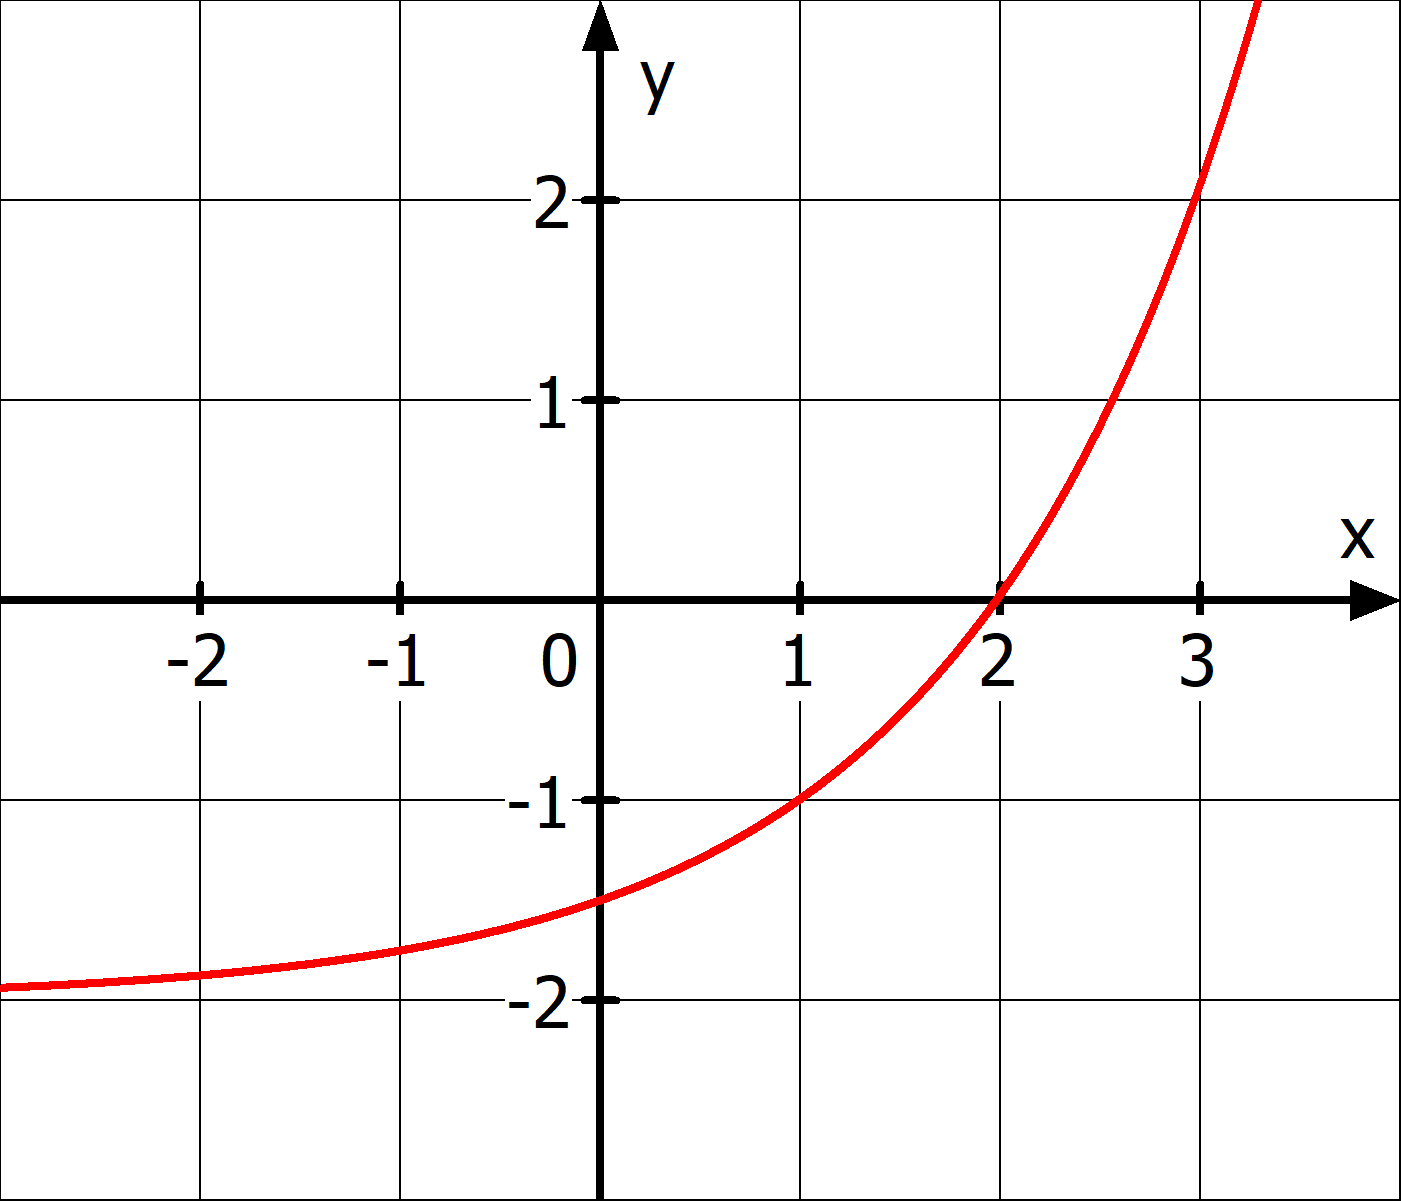
\includegraphics[width=.8\textwidth]{\ableitung/pics/ablSkizzierenF3.png}

            \vspace{0.1cm}

			\centering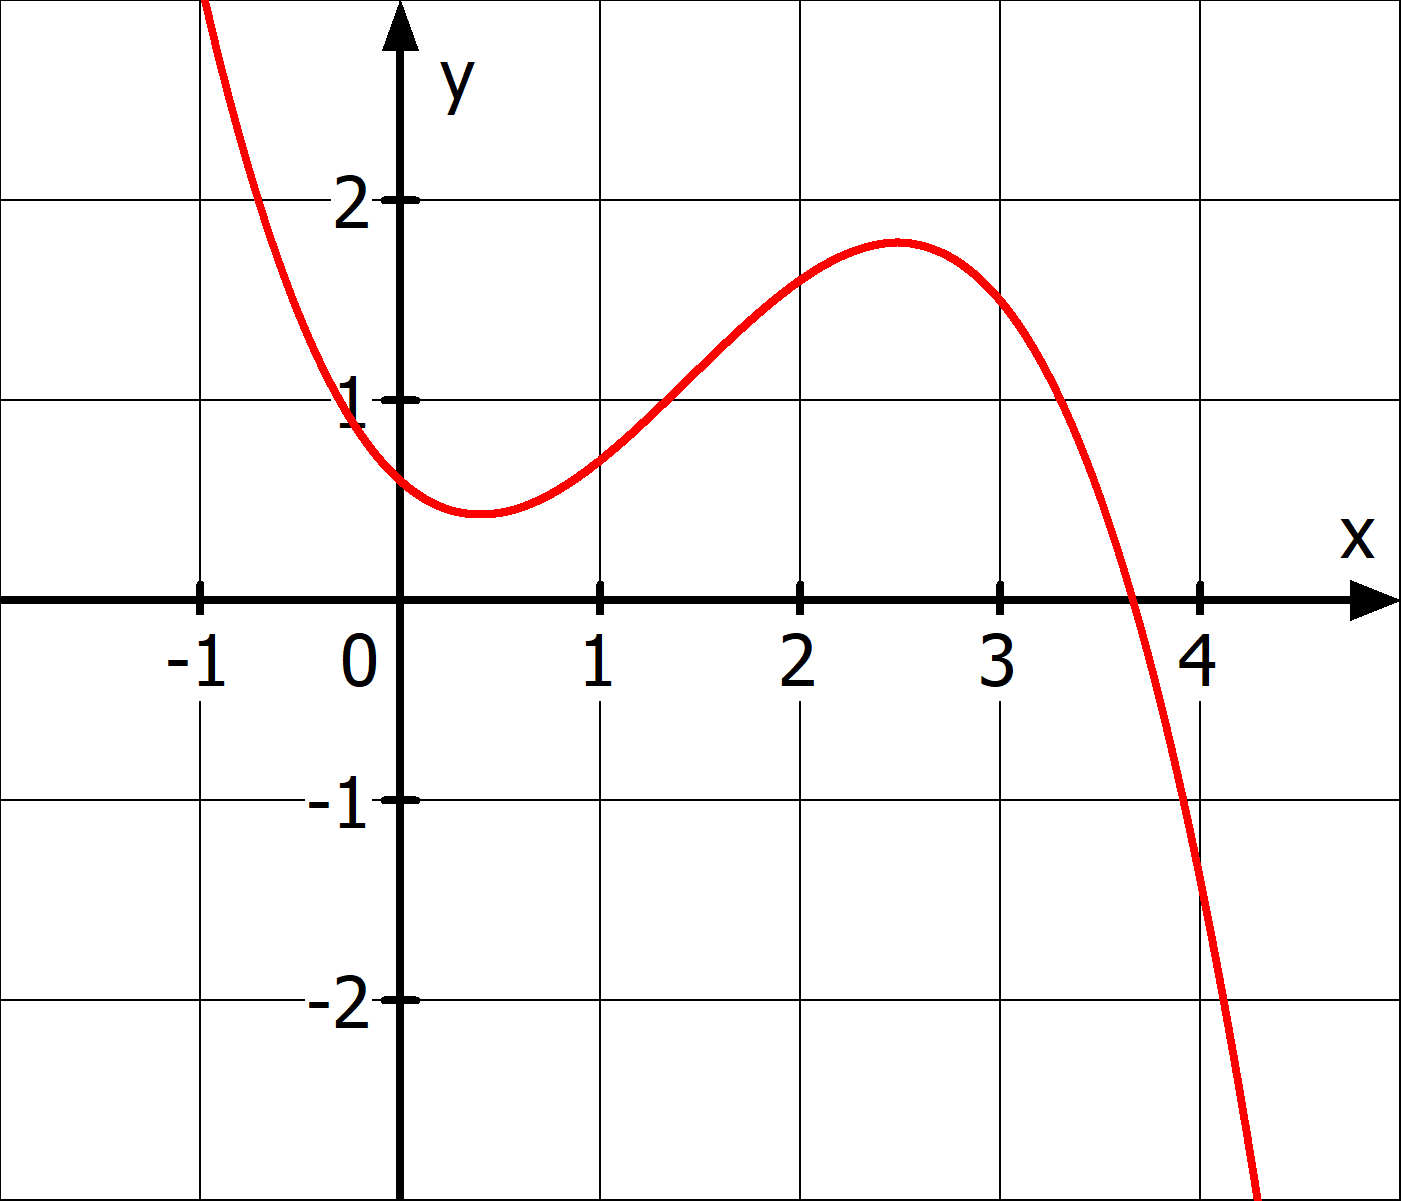
\includegraphics[width=.8\textwidth]{\ableitung/pics/ablSkizzierenF4.png}
		\end{minipage}%
		\begin{minipage}{0.5\textwidth}
			\centering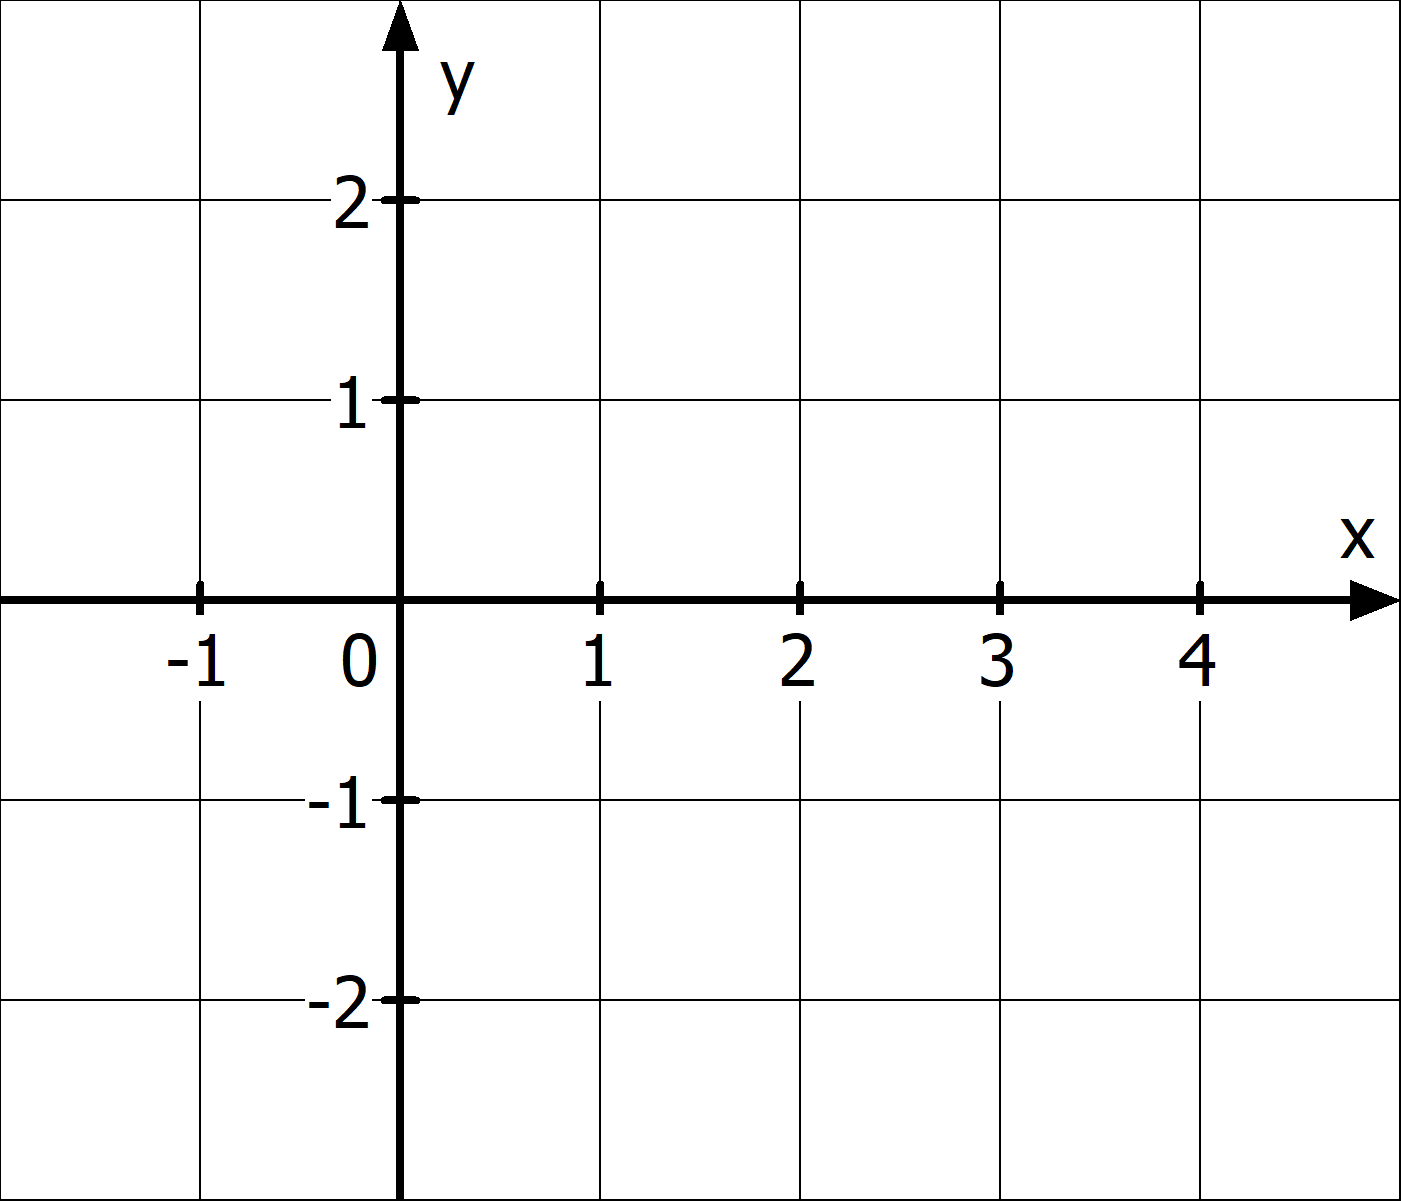
\includegraphics[width=.8\textwidth]{\ableitung/pics/ablSkizzierenE1.png}

            \vspace{0.1cm}

			\centering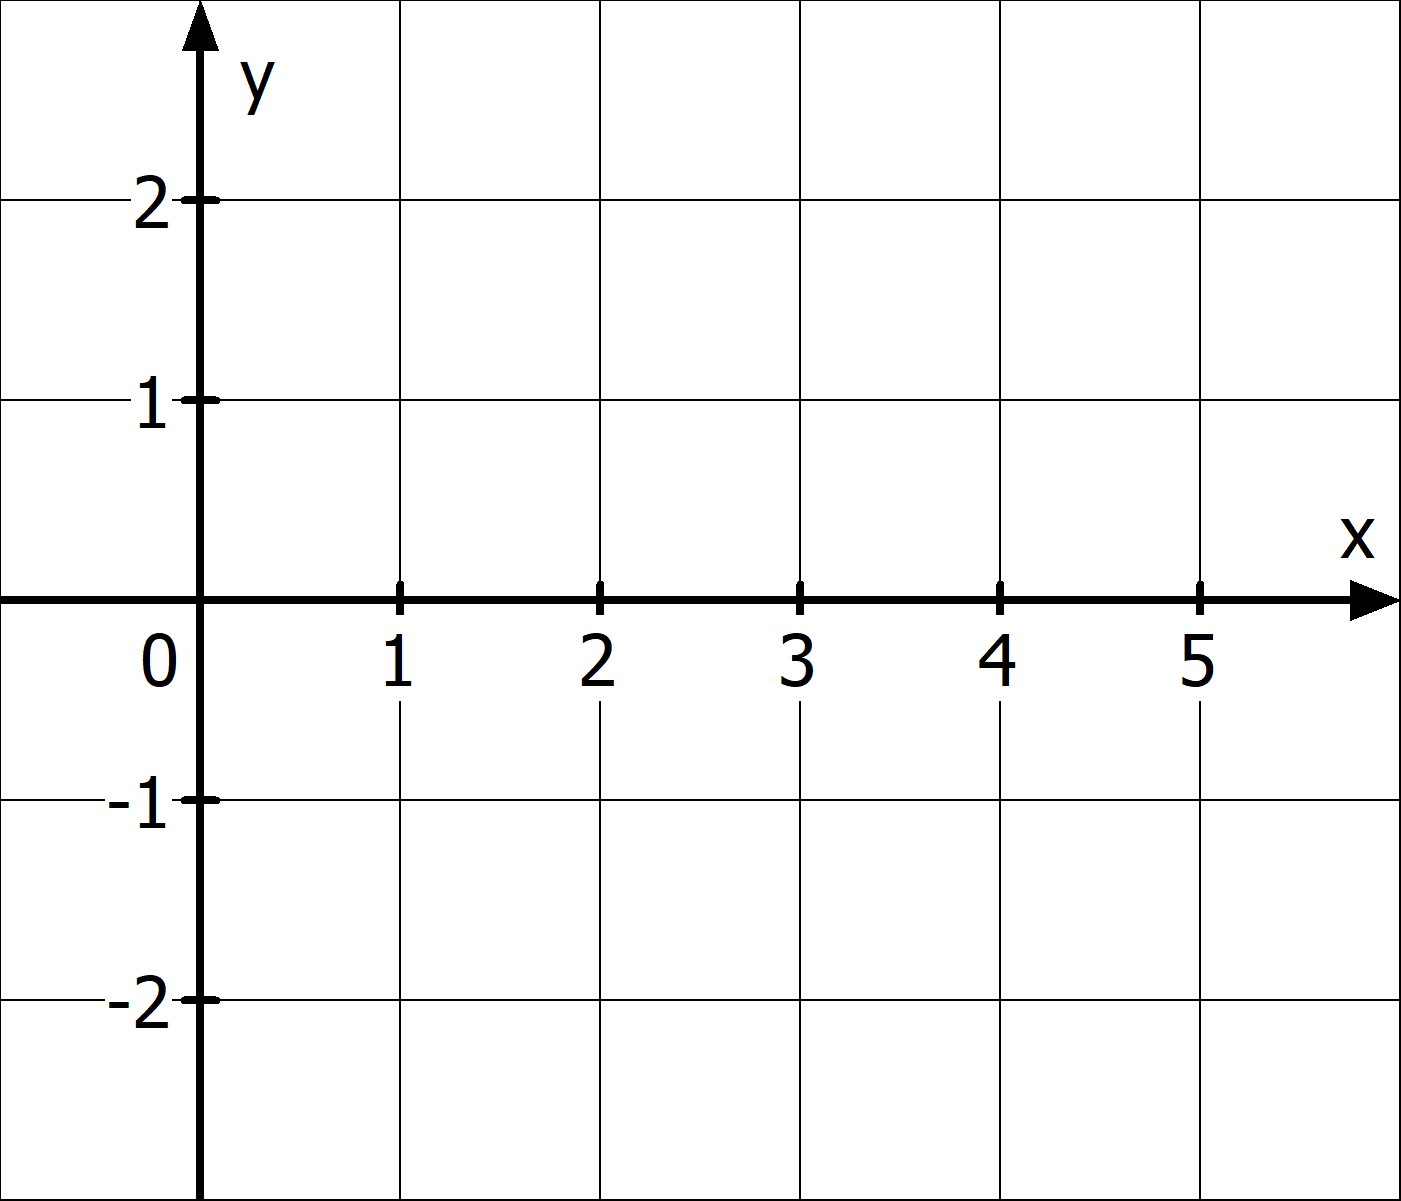
\includegraphics[width=.8\textwidth]{\ableitung/pics/ablSkizzierenE2.png}

            \vspace{0.1cm}

			\centering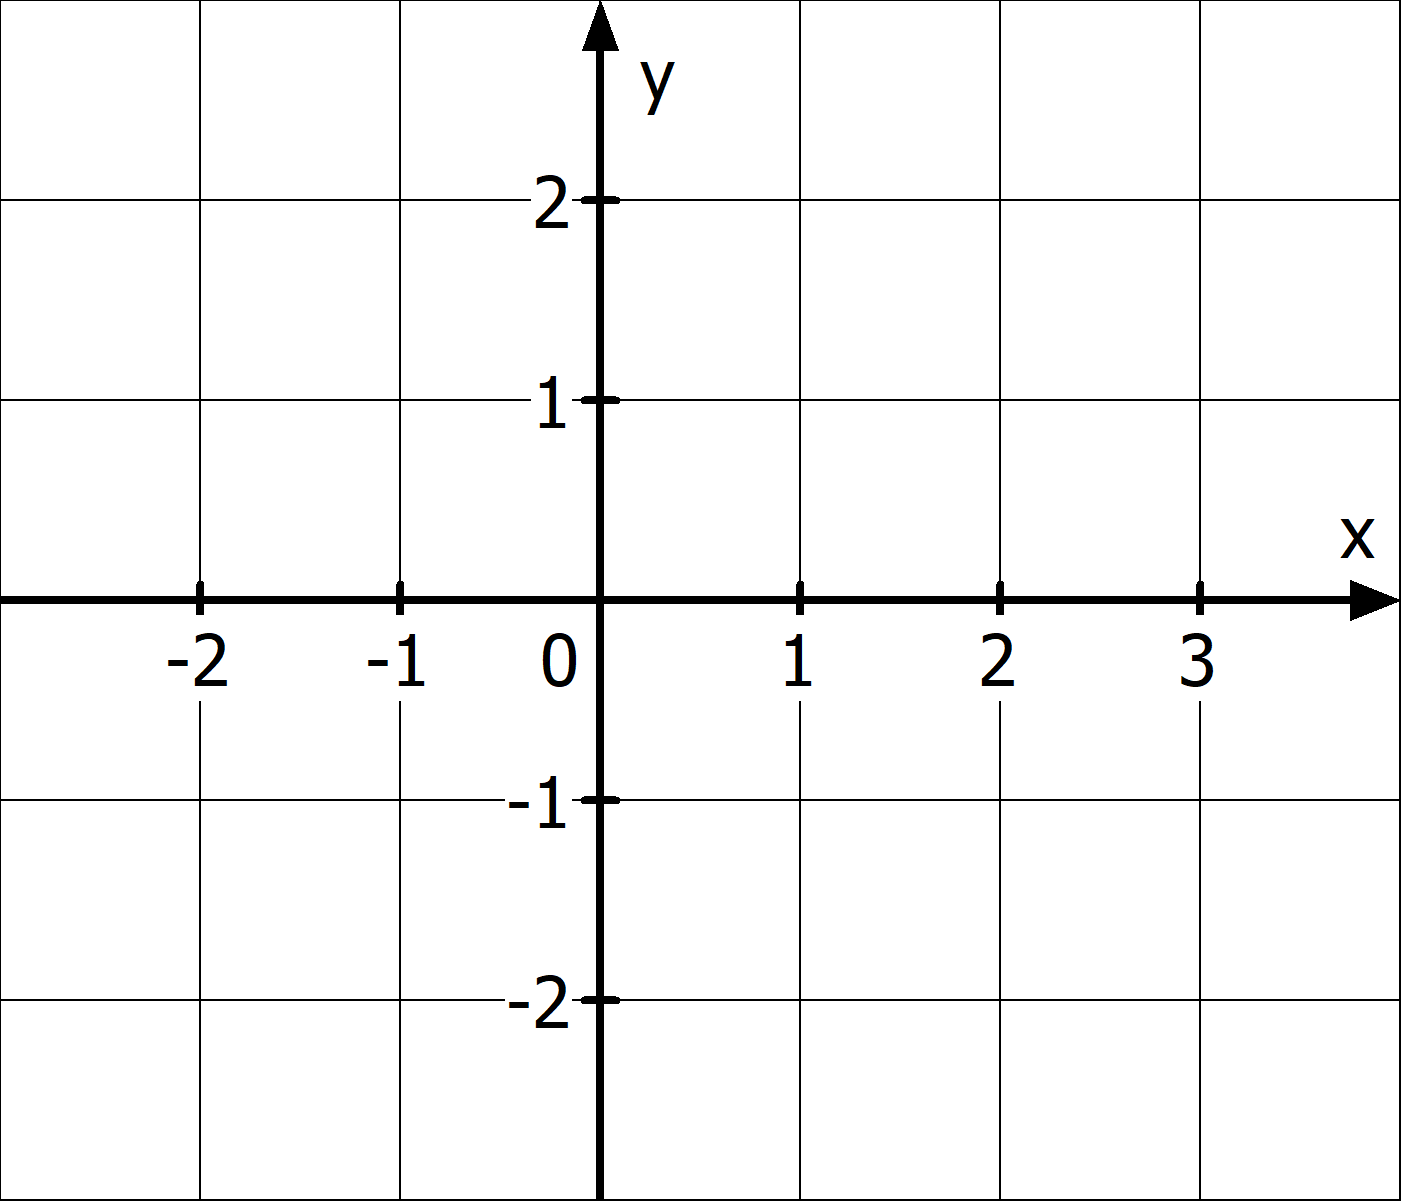
\includegraphics[width=.8\textwidth]{\ableitung/pics/ablSkizzierenE3.png}

            \vspace{0.1cm}

			\centering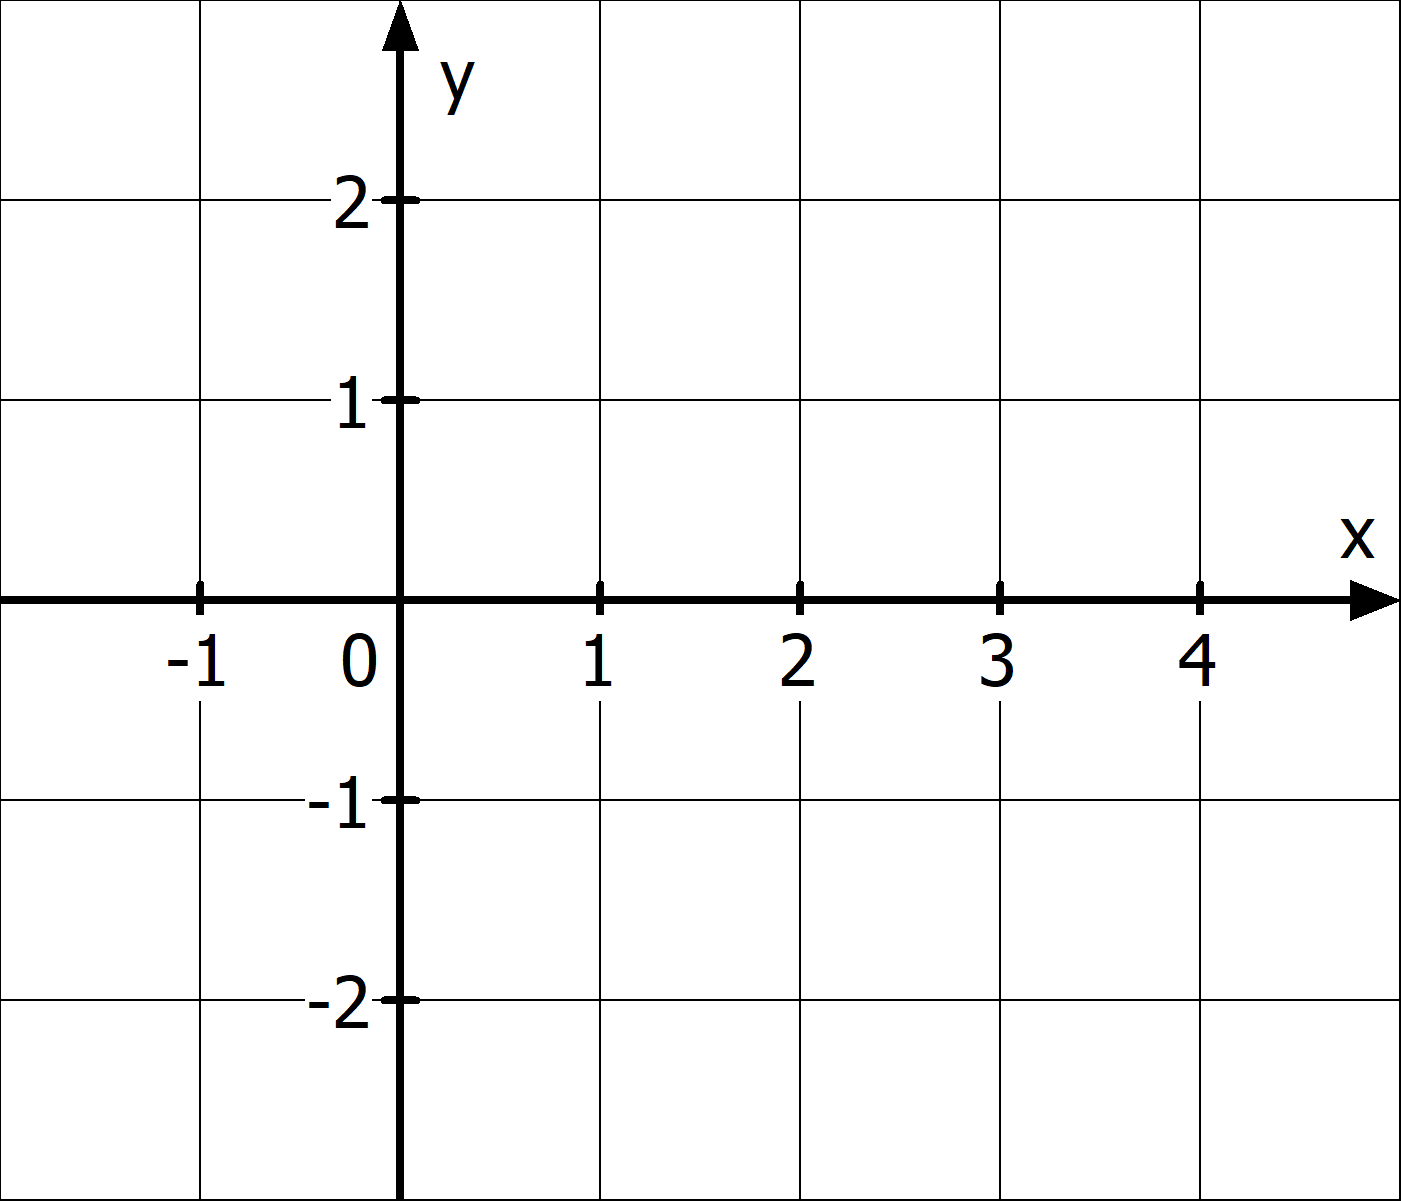
\includegraphics[width=.8\textwidth]{\ableitung/pics/ablSkizzierenE4.png}
		\end{minipage}%
	\end{minipage}
\end{Exercise}
\begin{Exercise}[title={\raggedright Zu sehen ist das Schaubild der Ableitung \(f'(x)\) einer Funktion \(f(x)\) mit dem Schaubild \(K_f\). Die Ableitungsfunktion hat den Grad 3. Kreuze die Aussagen an, die wahr sein müssen.}, label=ableitungInterpretationA1]

\bigskip

	\begin{minipage}{\textwidth}
		\adjustbox{valign=t}{\begin{minipage}{0.55\textwidth}
			\begin{itemize}
				\item[$\square$] \(K_f\) hat bei \(x=0\) eine waagrechte Tangente
				\item[$\square$] \(K_f\) hat mindestens eine Nullstelle
				\item[$\square$] \(K_f\) hat genau einen x-Wert, an dem die Tangente waagrecht ist.
				\item[$\square$] \(K_f\) hat auch positive Funktionswerte
				\item[$\square$] Es gilt \(f(-2)>f(-1)\)
				\item[$\square$] Es gilt \(f(x)>0\) für alle \(x\in\R\)
				\item[$\square$] \(K_f\) hat einen kleinsten Funktionswert (Tiefpunkt)

			\end{itemize}
		\end{minipage}}%
		\adjustbox{valign=t}{\begin{minipage}[][][c]{0.45\textwidth}
			\centering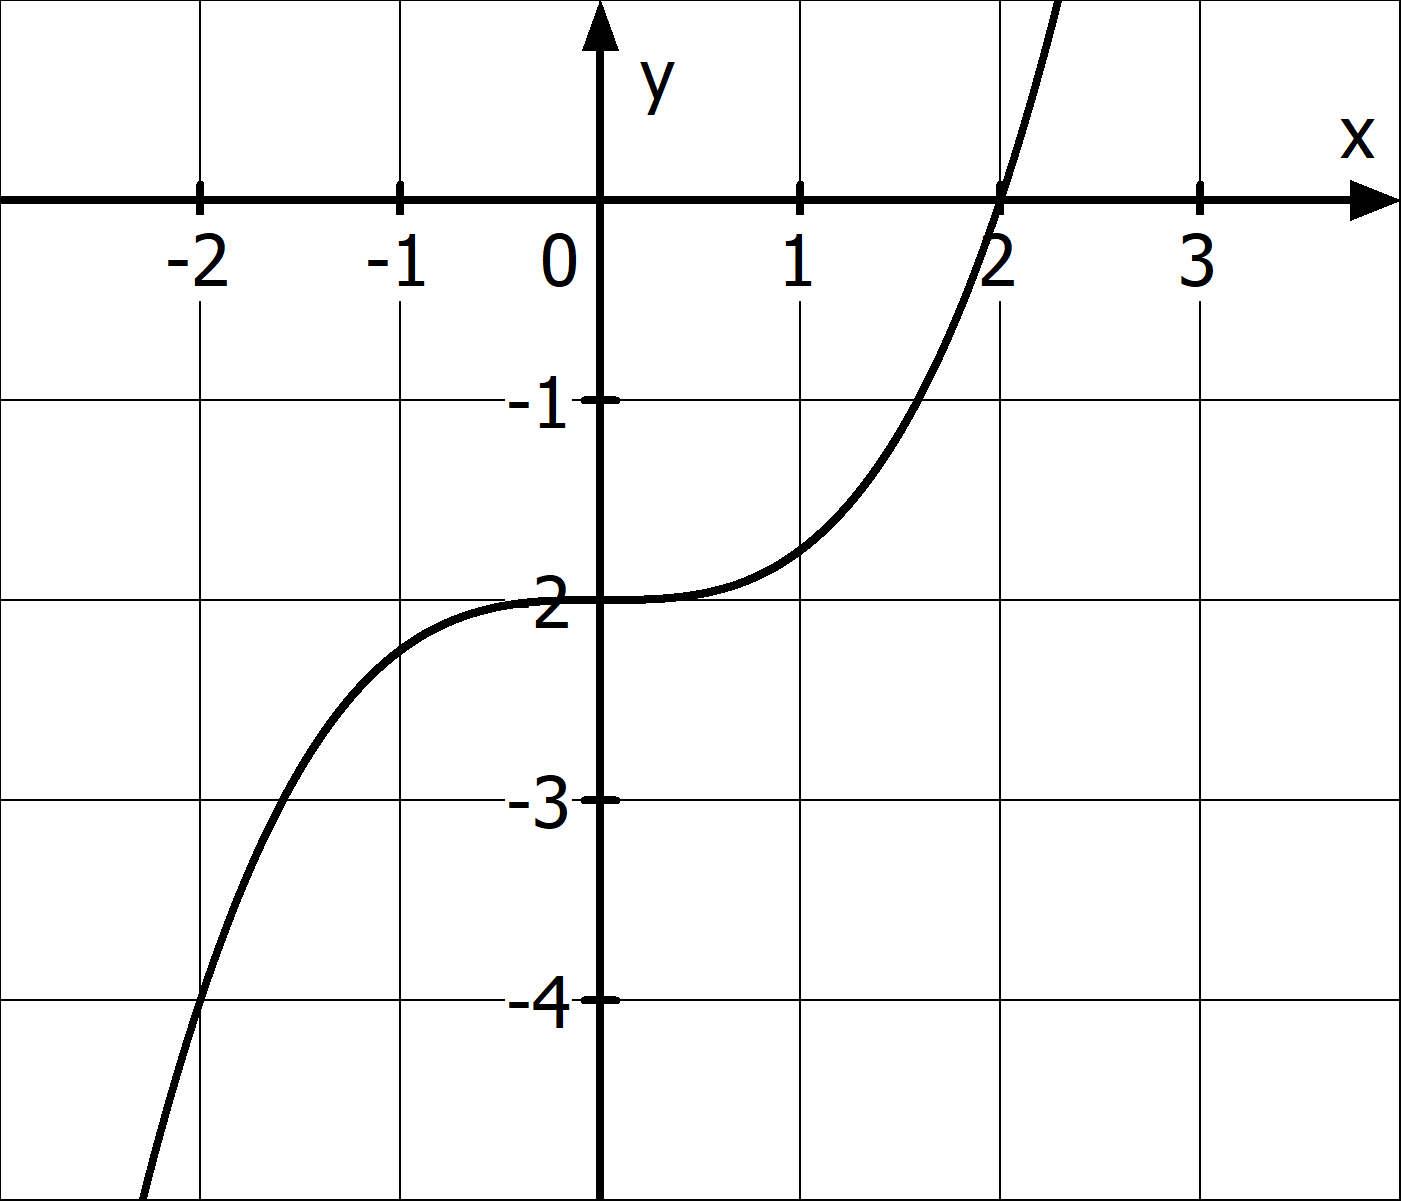
\includegraphics[width=\textwidth]{\ableitung/pics/interpretieren1.png}
		\end{minipage}}%
	\end{minipage}%
\end{Exercise}
%%%%%%%%%%%%%%%%%%%%%%%%%%%%%%%%%%%%%%%%%
\begin{Answer}[ref=schaubildZuordnenA1]

	\begin{minipage}{\textwidth}
		\begin{minipage}{0.5\textwidth}
			\centering Funktionen
		\end{minipage}%
		\begin{minipage}{0.5\textwidth}
			\centering Ableitungen
		\end{minipage}%

		\begin{minipage}{0.25\textwidth}
			\centering\(f(x)\)\vspace{0.2cm}

			\centering\(g(x)\)\vspace{0.2cm}

			\centering\(h(x)\)
		\end{minipage}%
		\begin{minipage}{0.25\textwidth}
			\centering\(j(x)\)\vspace{0.2cm}

			\centering\(k(x)\)\vspace{0.2cm}

			\centering\(l(x)\)
		\end{minipage}%
		\begin{minipage}{0.25\textwidth}
			\centering\(h'(x)\)\vspace{0.2cm}

			\centering\(g'(x)\)\vspace{0.2cm}

			\centering\(l'(x)\)
		\end{minipage}%
		\begin{minipage}{0.25\textwidth}
			\centering\(f'(x)\)\vspace{0.2cm}

			\centering\(j'(x)\)\vspace{0.2cm}

			\centering\(k'(x)\)
		\end{minipage}%
	\end{minipage}%
\end{Answer}
\begin{Answer}[ref=ableitungSkizzierenA1]

	\begin{minipage}{\textwidth}
		\begin{minipage}{0.5\textwidth}
			\adjustbox{valign=t, padding = 0ex 0ex 1ex 0ex }{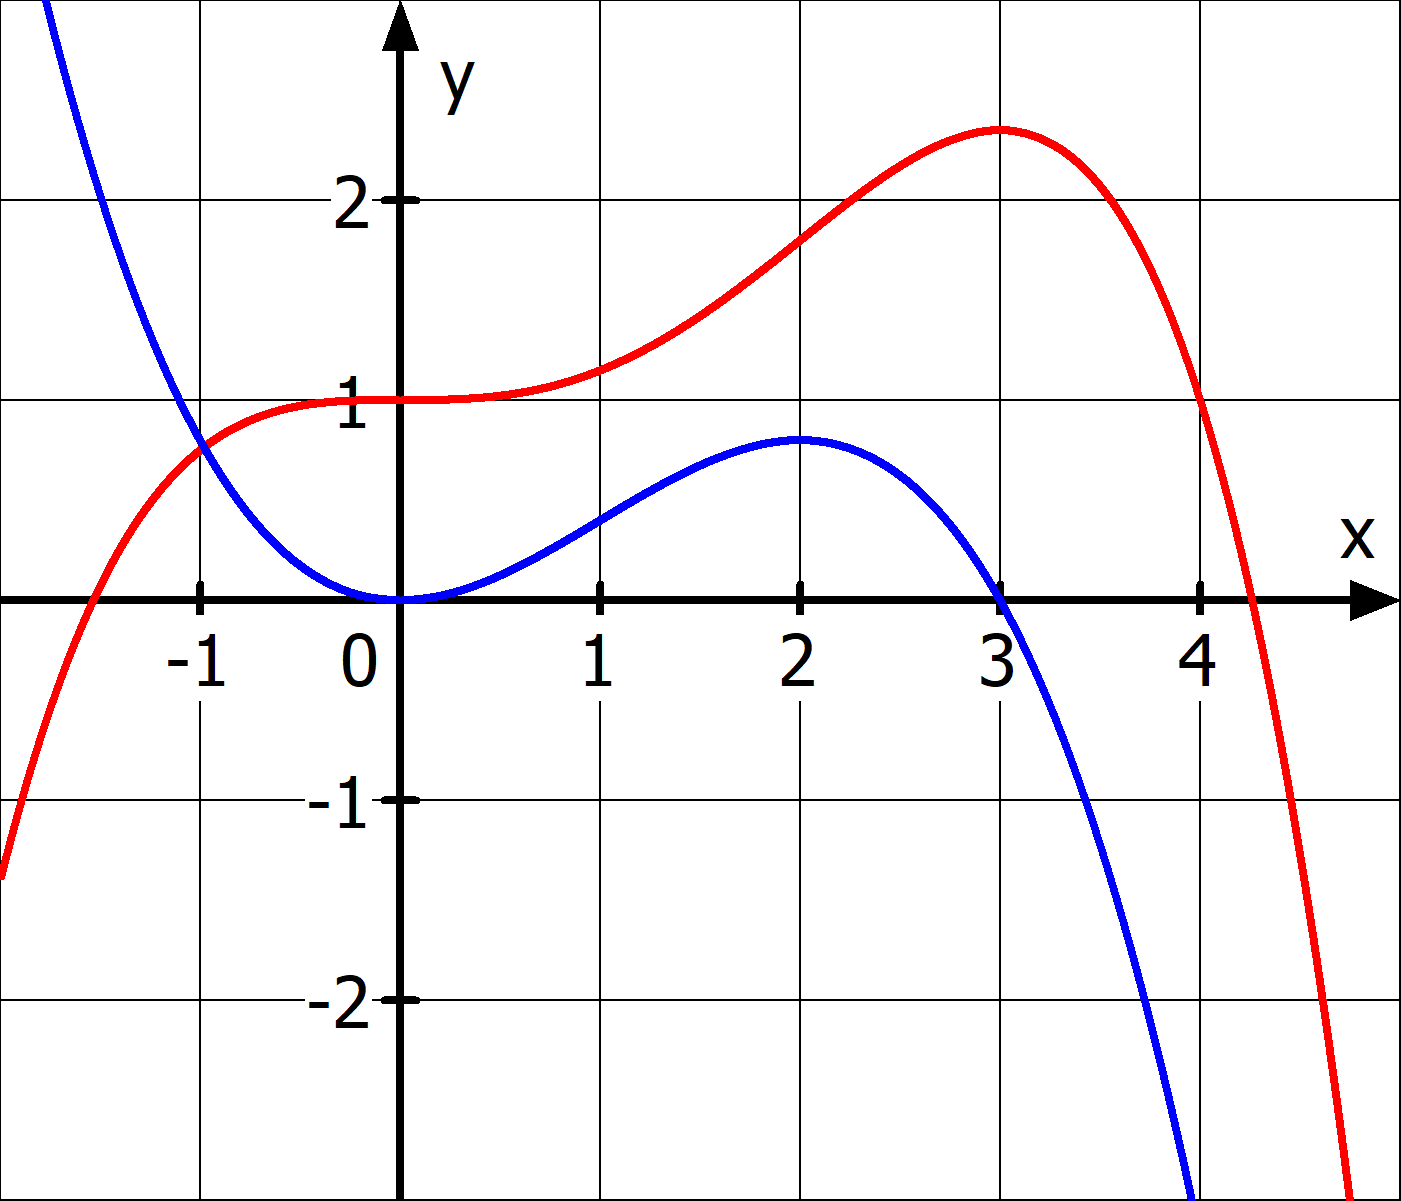
\includegraphics[width=\textwidth-1ex]{\ableitung/pics/ablSkizzierenL1.png}}%

            \vspace{2ex}

			\adjustbox{valign=t, padding = 0ex 0ex 1ex 0ex }{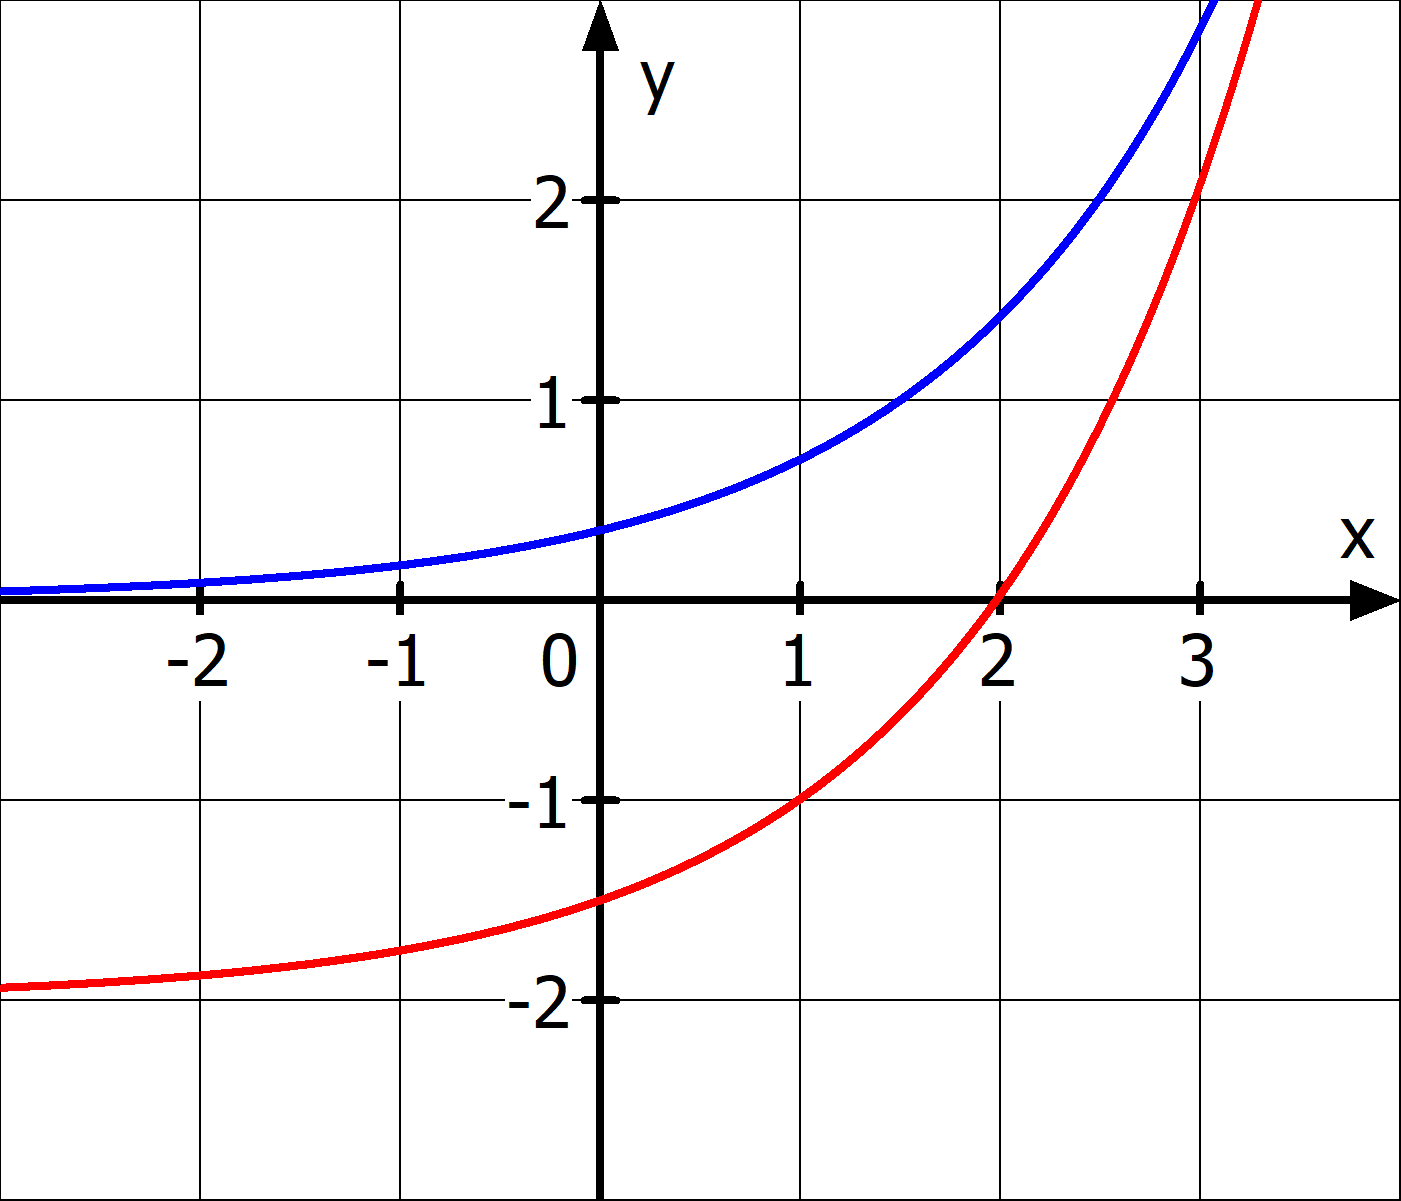
\includegraphics[width=\textwidth-1ex]{\ableitung/pics/ablSkizzierenL3.png}}%
		\end{minipage}%
		\begin{minipage}{0.5\textwidth}
			\adjustbox{valign=t, padding = 1ex 0ex 0ex 0ex }{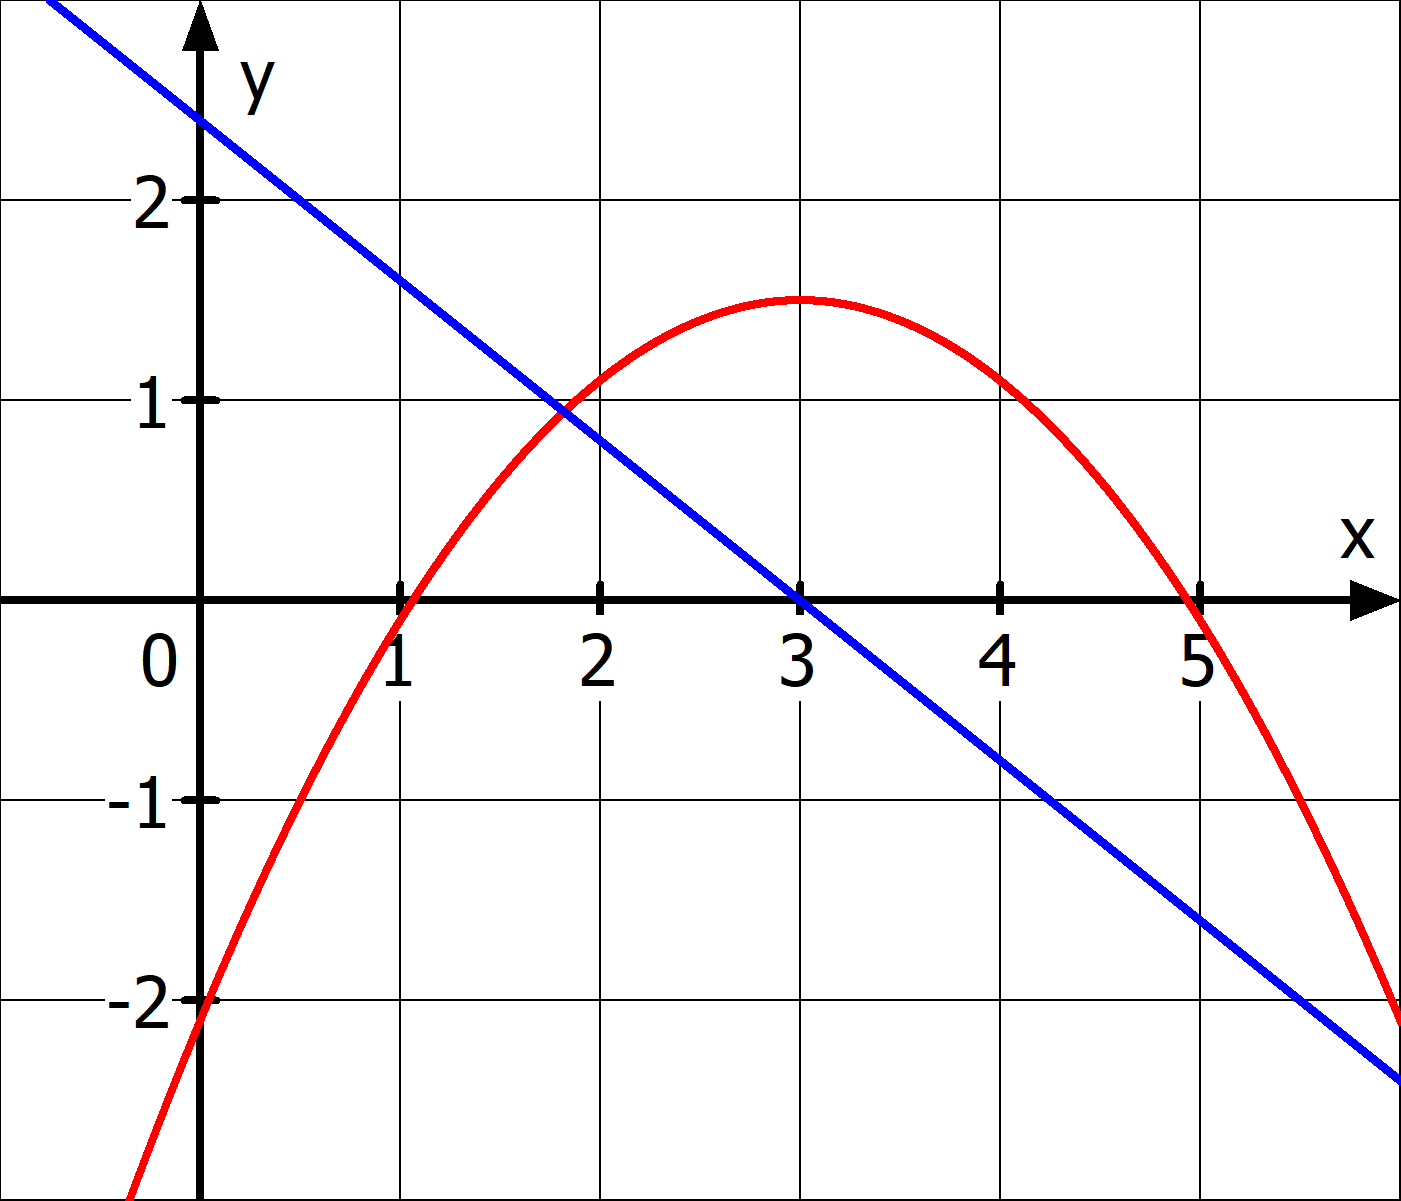
\includegraphics[width=\textwidth-1ex]{\ableitung/pics/ablSkizzierenL2.png}}%

            \vspace{2ex}

			\adjustbox{valign=t, padding = 1ex 0ex 0ex 0ex }{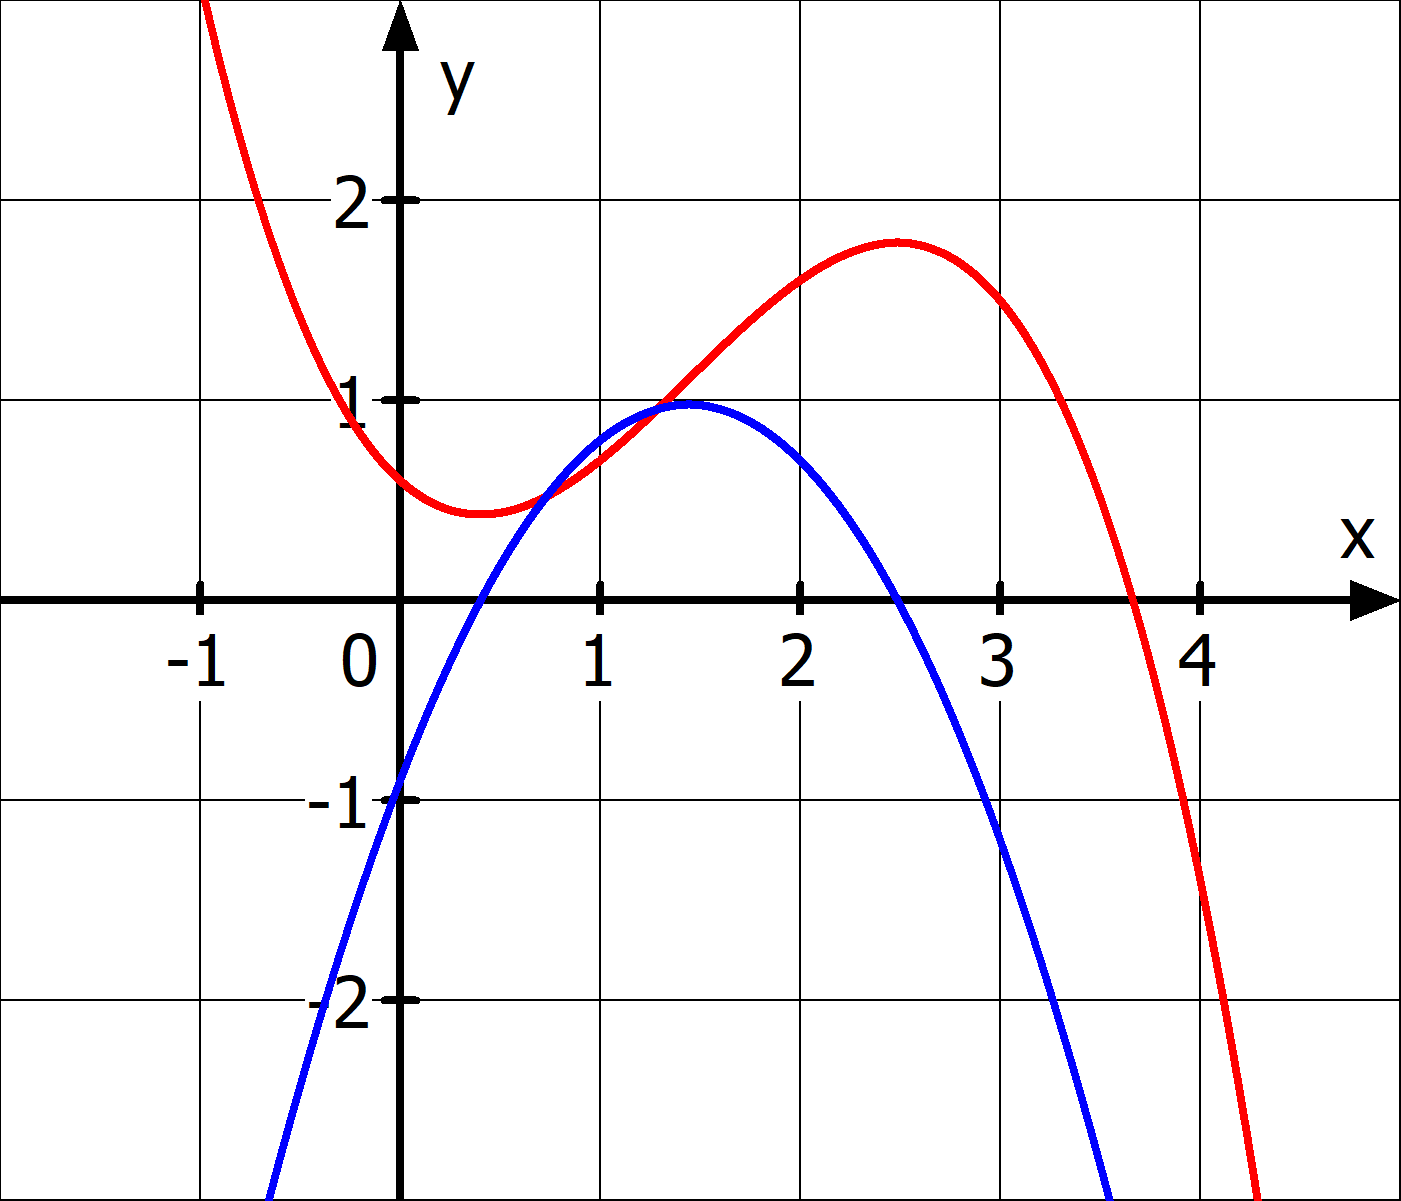
\includegraphics[width=\textwidth-1ex]{\ableitung/pics/ablSkizzierenL4.png}}%
		\end{minipage}
	\end{minipage}%

    \bigskip

	Hinweis: Grundsätzlich muss die Ableitung positiv sein, wenn die Funktion steigt bzw. negativ, wenn die Funktion fällt. Zusätzlich kann man an ein paar Stellen mit Hilfe der Tangente den Wert der Ableitung schätzen.
\end{Answer}
\begin{Answer}[ref=ableitungInterpretationA1]

	\begin{itemize}
		\item[$\square$] \(K_f\) hat bei \(x=0\) eine waagrechte Tangente

		Da \(f'(0)=-2\neq 0\) gilt, ist die Tangente fallend mit Steigung -2 und nicht waagrecht (Steigung 0).
		\item[$\square$] \(K_f\) hat mindestens eine Nullstelle

		Da die Ableitung den Grad 3 hat, hat \(f(x)\) den Grad 4. Funktionen vom Grad 4 können NST haben, müssen aber nicht, daher ist die Aussage nicht immer wahr.
		\item[$\checkmark$] \(K_f\) hat genau einen x-Wert, an dem die Tangente waagrecht ist.

		Die Ableitung hat genau eine NST.
		\item[$\checkmark$] \(K_f\) hat auch positive Funktionswerte

		Da \(f'(x)\xrightarrow{\hphantom{\ }x\to\infty\hphantom{\ }}\infty\) gilt, steigt \(K_f\) ab \(x=2\) immer steiler und muss daher auch irgendwann in den positiven Bereich gehen.
		\item[$\checkmark$] Es gilt \(f(-2)>f(-1)\)

		Da die Ableitung im Bereich von \(x=-2\) bis \(x=-1\) negativ ist, fällt \(K_f\) in diesem Bereich, d.h. die Funktionswerte links sind größer als die rechts.
		\item[$\square$] Es gilt \(f(x)>0\) für alle \(x\in\R\)

		Wir können \(K_f\) beliebig in y-Richtung verschieben ohne die Ableitung zu ändern, d.h. dass \(K_f\) auch negative Funktionswerte bzw. NST haben kann.
		\item[$\checkmark$] \(K_f\) hat einen kleinsten Funktionswert (Tiefpunkt)

		Für \(x<2\) ist die Ableitung negativ, d.h. \(K_f\) fällt. Für \(x>2\) ist die Ableitung positiv, d.h. \(K_f\) steigt. Daraus folgt, dass bei \(x=2\) der Funktionswert am kleinsten ist und \(K_f\) einen Tiefpunkt hat.
	\end{itemize}
\end{Answer}